% !TeX TS-program = pdflatex
% !TeX encoding = UTF-8
% !TeX spellcheck = en_GB
% !TeX root = contest-main.tex
\documentclass[]{beamer}

\usepackage[T1]{fontenc}
\usepackage{textcomp}
\usepackage[utf8]{inputenc}
\usepackage{babel}
%\geometry{}

\graphicspath{{../r/plots/},{./Figures/}}

\usepackage{booktabs}
%\usepackage{caption}
%\captionsetup{format=hang,labelsep=colon}%,font={small,rm},labelfont={sf,bf}}
%\captionsetup[table]{skip=-0.9\medskipamount,position=top}

\usepackage[ruled,linesnumbered]{algorithm2e}
\SetNlSty{texttt}{}{}
\SetKw{Or}{or}
\SetKw{And}{and}
\SetKw{Not}{not}

% -------- %
\title{Diagnosing Diabetes}
\subtitle{Comparison between Logistic regression and Ensemble trees}
\author{Francesco Marchini \and Alessandra Spinaci \and David Nardi}
\institute[UniFi]{MSc in AI, University of Florence}
\date{May 21, 2024}
%\logo{\includegraphics[width=0.2\textwidth]{./Figures/logo}}
%\titlegraphic{\includegraphics{./Figures/logo}}
% -------- %

\usepackage{appendixnumberbeamer}
%\mode<presentation>
\usetheme[progressbar=foot,numbering=counter]{metropolis}
%\useoutertheme[right]{sidebar}
\setbeamercovered{dynamic}
%\setbeamertemplate{blocks}[default]%[shadow=true]
\setbeamertemplate{sections/subsections in toc}[circle]
\setbeamertemplate{items}[circle]
\setbeamertemplate{navigation symbols}{}
\metroset{block=fill}

%\mode<all>

% definizione degli enunciati matematici
%\theoremstyle{definition}
%\newtheorem{defs}{Definition}
%\theoremstyle{plain}
%\newtheorem{thm}{Theorem}

\usepackage{mathtools}
\newcommand{\numberset}{\mathbb}
\newcommand{\R}{\numberset{R}}
\DeclareMathOperator{\sign}{sign}
\DeclareMathOperator*{\argmin}{arg\,min}
\DeclarePairedDelimiter{\abs}{\lvert}{\rvert}
\DeclarePairedDelimiter{\norma}{\lVert}{\rVert}
\DeclarePairedDelimiter{\set}{\{}{\}}
\renewcommand{\epsilon}{\varepsilon}

\usepackage{subfig}

\usepackage{siunitx}
\sisetup{%
	output-decimal-marker={.},group-separator={\,},%
	%	round-mode=places,round-precision=6,%
	table-parse-only,table-number-alignment=center%
}

%\usepackage{enumitem}

\usepackage{pgfplots} % + tikz
\pgfplotsset{compat=newest}
\usetikzlibrary{shapes,calc}

\tikzstyle{cloud} = [draw,ellipse,centered,text width=3.5em,text centered,
					inner sep=0.5pt,outer sep=0pt,fill=mLightBrown!20,font=\footnotesize]
\tikzstyle{cloud2} = [draw,ellipse,centered,text width=3em,text centered,
					  inner sep=1.5pt,outer sep=0pt,fill=mLightBrown!20,font=\small]

\tikzstyle{treenode} = [draw,circle,minimum width=1.4em,font=\footnotesize,text centered,
						inner sep=1.2pt,outer sep=0pt]

\tikzstyle{immagine} = [above right,inner sep=0pt,outer sep=0pt]

%\tikzset{},
%	testo/.style={fill=white,align=center,fill opacity=0,text opacity=1,below right,
%		font=\scriptsize},
%	testo1/.style={fill=white,align=center,fill opacity=0,text opacity=1,below right,
%		font=\tiny},
%	testo2/.style={fill=white,align=center,fill opacity=0,text opacity=1,above right,
%		font=\tiny}}

\newcommand{\maxlike}{{\tiny ML}}

% ------------------------------- %
\usepackage{listings}
\definecolor{Rkwd}{rgb}{0.737,0.353,0.396}
\definecolor{Rparam}{rgb}{0.333,0.667,0.333}
\definecolor{Rnum}{rgb}{0.686,0.059,0.569}
\definecolor{Rstr}{rgb}{0.192,0.494,0.8}
\definecolor{Rcomm}{rgb}{0.678,0.584,0.686}
% R
\lstdefinestyle{Rlang}{language=R,%
	keywordstyle=\color{Rkwd},basicstyle=\small\ttfamily,%
	commentstyle=\color{Rcomm}\ttfamily\em,%
	stringstyle=\color{Rstr}\rmfamily,%
	numbers=left,numberstyle=\tiny\color{green},stepnumber=1,numbersep=5pt,%
	showstringspaces=false,breaklines=true,frameround=ftff,%
	frame=lines,backgroundcolor=\color{lightergray},firstnumber=last,%
	deletekeywords={data,model},%
	morekeywords={TRUE,FALSE,NULL},%
}
\lstset{style=Rlang,escapeinside={£!}{!£}}
% ------------------------------- %

%\usepackage{pgfpages}
%\pgfpagesuselayout{4 on 1}[a4paper,border shrink=5mm,landscape]
%\usepackage{showframe}
\begin{document}

\pdfbookmark[1]{Title page}{cover}
\maketitle

% ------------------------------- %
\begin{frame}{Introduction - Dataset Diabetes}
    Variables
    \begin{itemize}
        \item Pregnancies: Number of times pregnant
        \item Glucose: Plasma glucose concentration a 2 hours in an oral glucose tolerance test
        \item BloodPressure: Diastolic blood pressure (mmHg)
        \item SkinThickness: Triceps skin fold thickness (mm)
        \item Insulin: 2-Hour serum insulin (mu U/ml)
        \item BMI: Body mass index (weight in kg/(height in m)\^2)
        \item DiabetesPedigreeFunction: Diabetes pedigree function
        \item Age: Age (years)
        \item Outcome: Class variable (0 or 1)
    \end{itemize}
\end{frame}

\begin{frame}{Introduction - Goal}
    Make binary classification in order to predict diabetes positivity using different methods and compare them     
\end{frame}

\begin{frame}{Introduction - Methods}
    Used methods to predict diabetes
    \begin{itemize}
        \item Shrinked Logistic Regression
        \begin{itemize}
            \item Lasso
            \item Ridge
            \item ElasticNet
            \item Adaptive Lasso
        \end{itemize}
        \item Random Forest
        \item Boosting
        \begin{itemize}
            \item Adaboost
            \item Stochastic Setting 
        \end{itemize}
    \end{itemize}
\end{frame}

\begin{frame}{Introduction - Data Preprocessing}
    Removing null values by replacing them with mean value
\end{frame}

\begin{frame}{Logistic Regression package}

\begin{columns}[T]
\begin{column}{0.5\textwidth}
TODO -- Formact code

\texttt{alpha = 1   \# Lasso = 1 -- Ridge = 0 -- 0 < Elastic < 1}
\texttt{cv.model = cv.glmnet(x.train, y.train, family = 'binomial', alpha = alpha)}
\texttt{best.lambda <- cv.model\$lambda.min}
\end{column}
\begin{column}{0.5\textwidth}
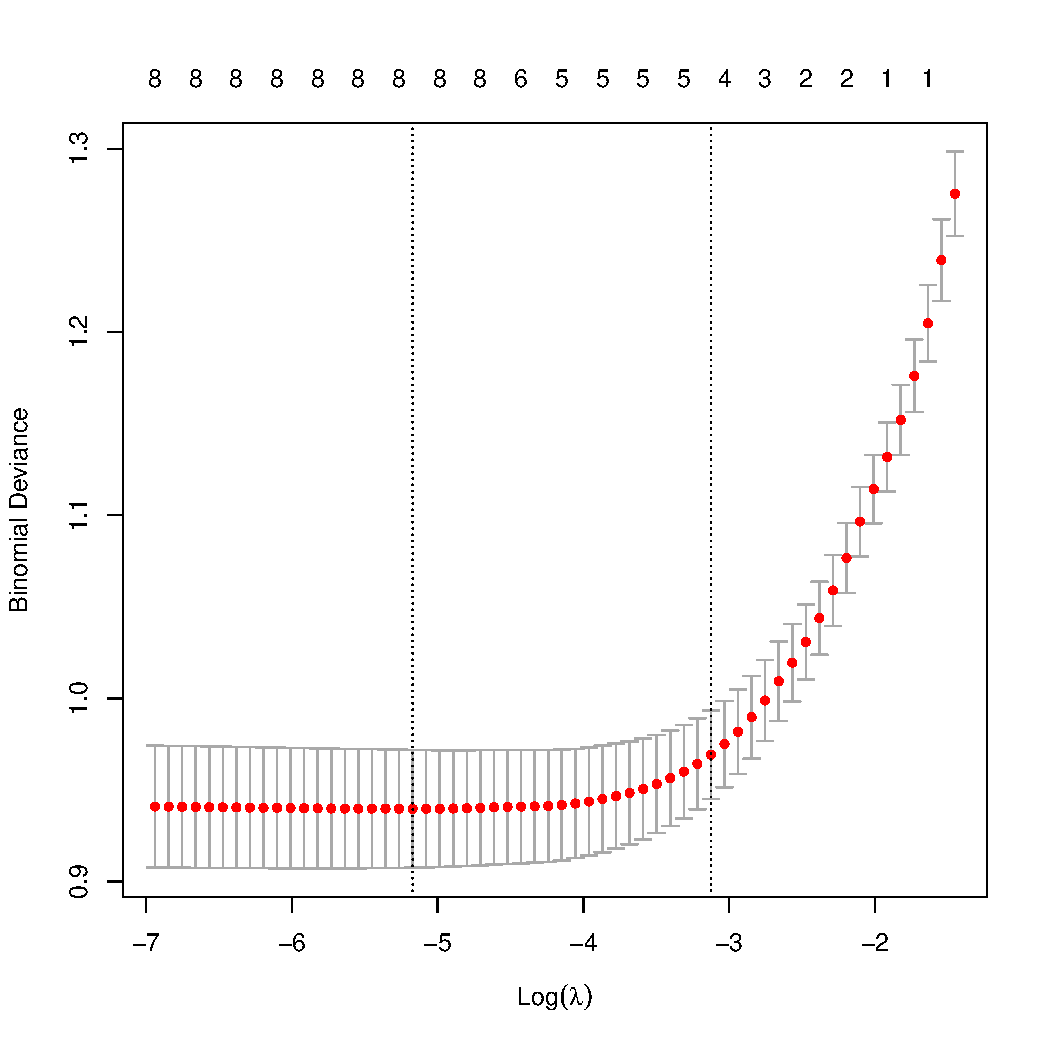
\includegraphics[width=0.85\columnwidth]{./Figures/logist/cv_lambda.pdf}
\end{column}
\end{columns}

\end{frame}

\begin{frame}{Ridge and Lasso variable importance}

\vspace*{-1em}\begin{columns}[T]
\begin{column}{0.5\textwidth}
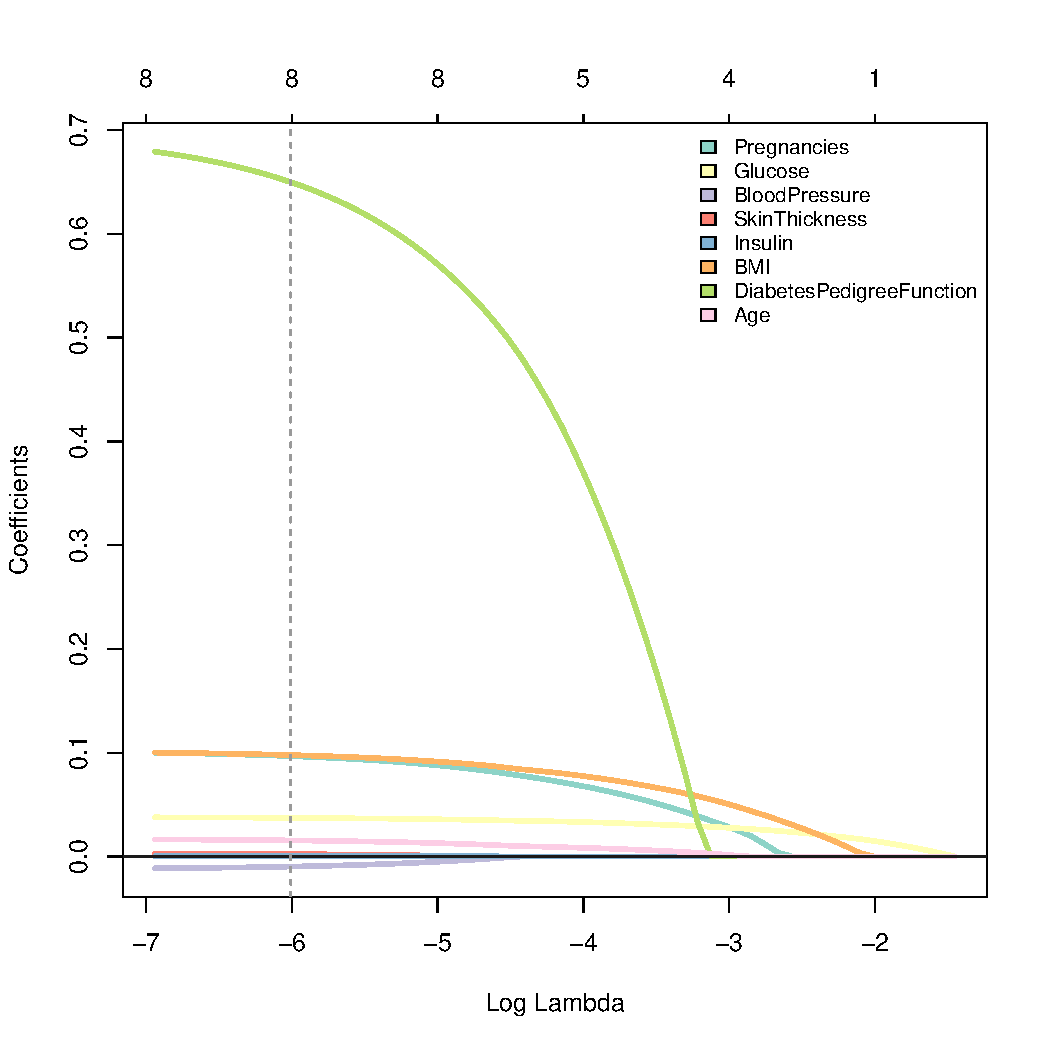
\includegraphics[width=0.85\columnwidth]{./Figures/logist/diabetes_lasso.pdf}
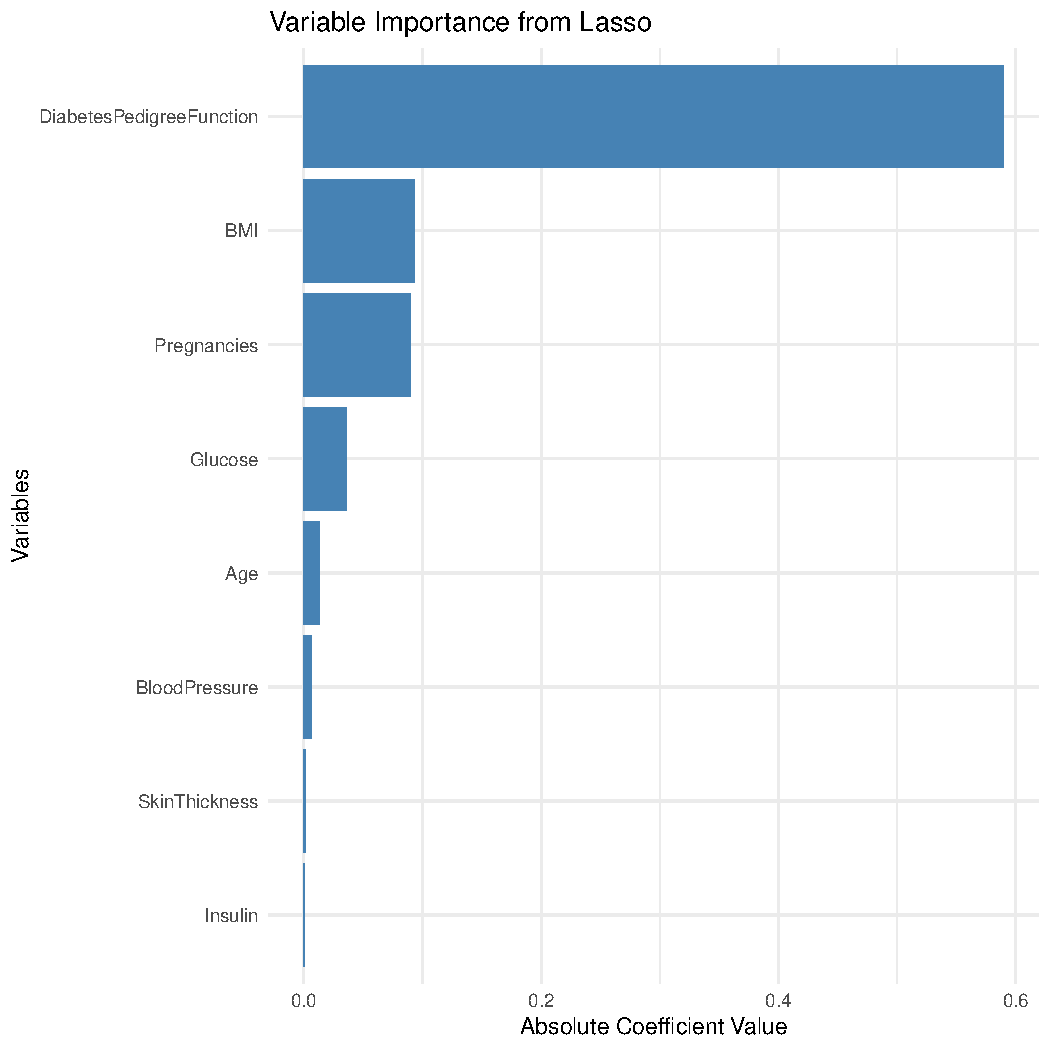
\includegraphics[width=0.7\columnwidth]{./Figures/logist/variable_importance_lasso.pdf}
\end{column}
\begin{column}{0.5\textwidth}
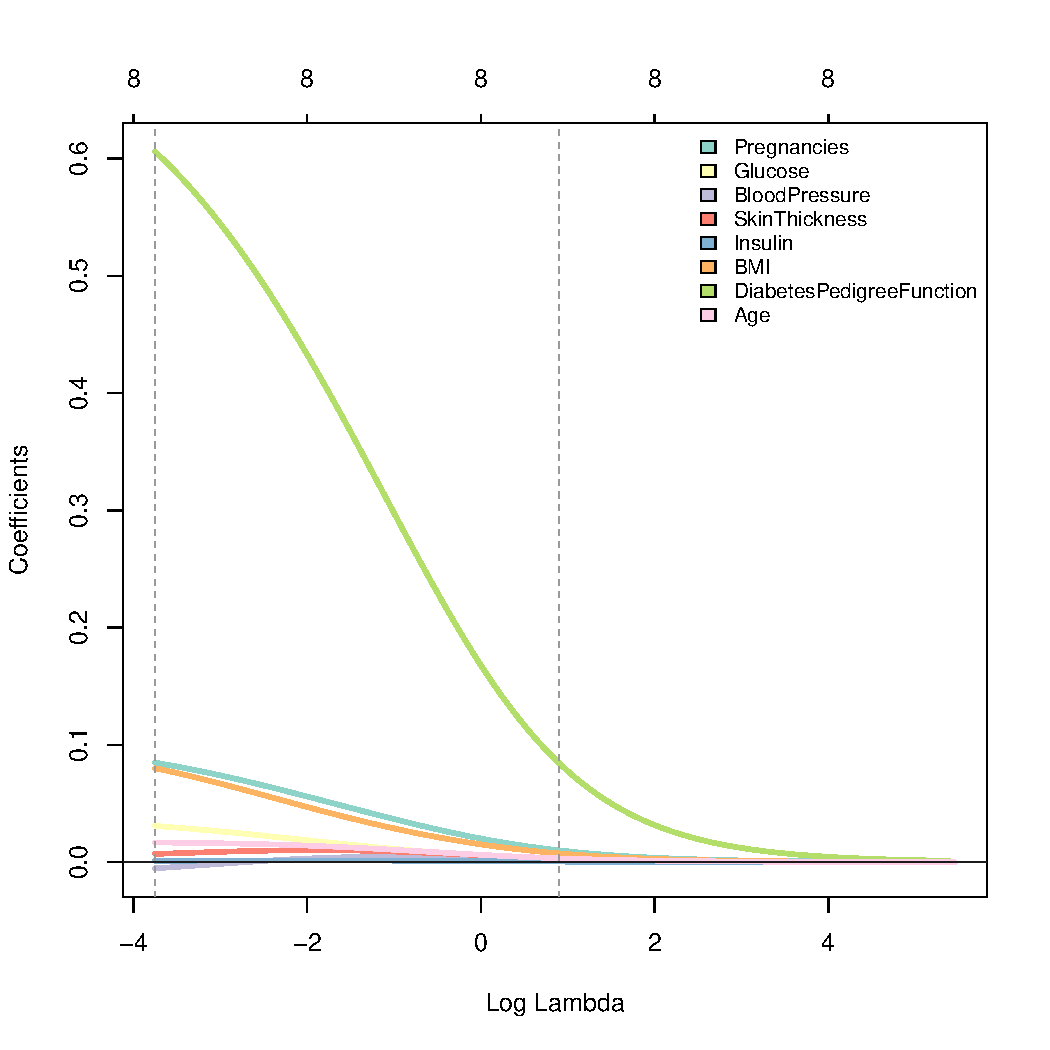
\includegraphics[width=0.85\columnwidth]{./Figures/logist/diabetes_ridge.pdf}
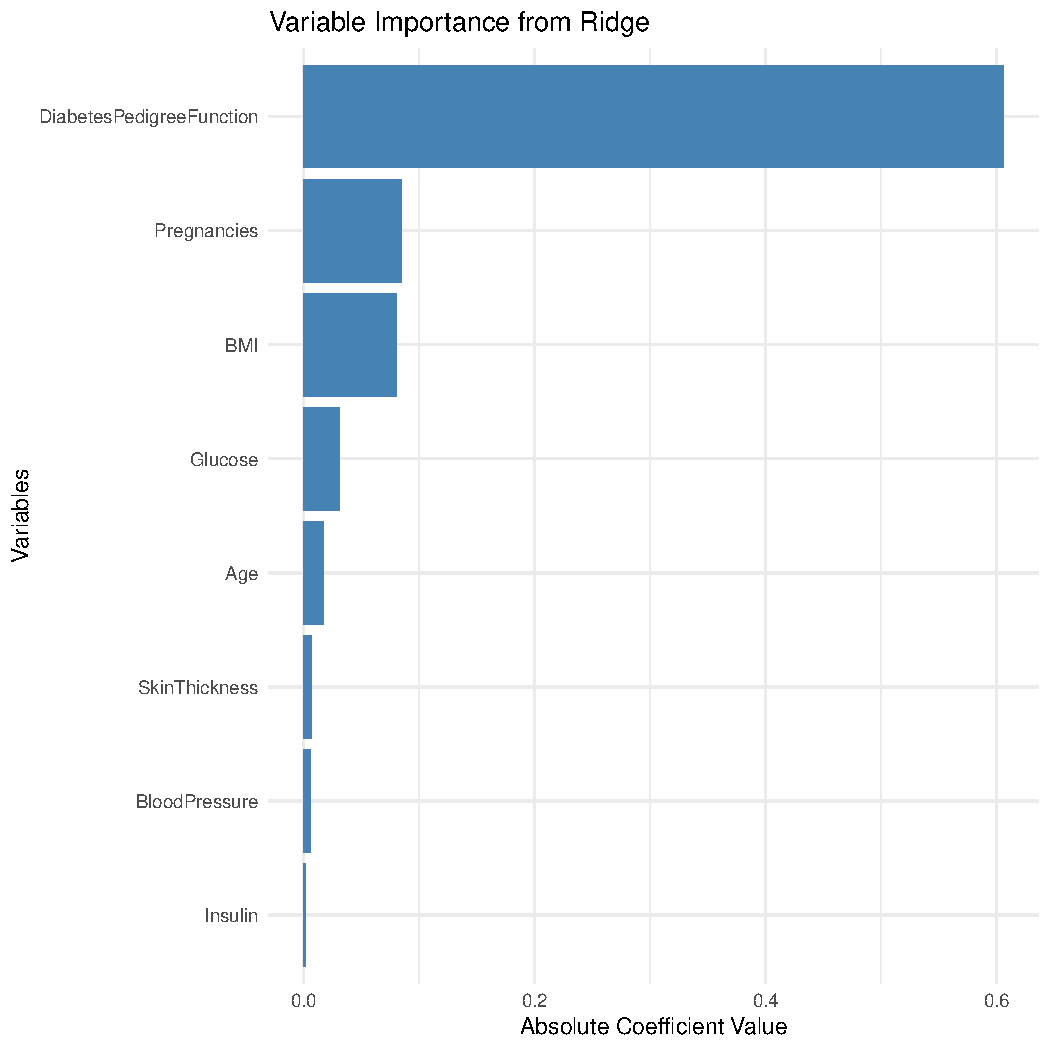
\includegraphics[width=0.7\columnwidth]{./Figures/logist/variable_importance_ridge.pdf}
\end{column}
\end{columns}

\end{frame}

\begin{frame}{ElasticNet and AdaLasso variable importance}

\vspace*{-1em}\begin{columns}[T]
\begin{column}{0.5\textwidth}
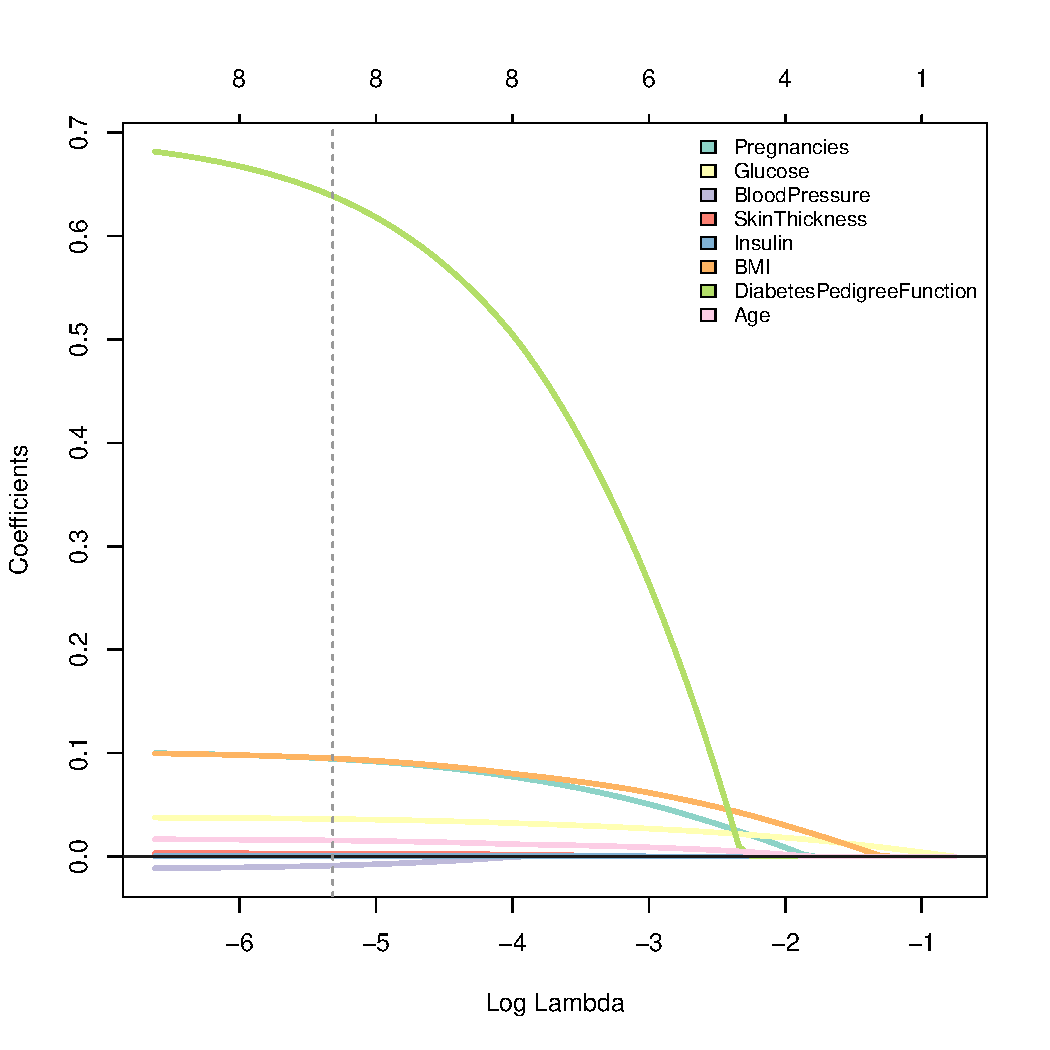
\includegraphics[width=0.85\columnwidth]{./Figures/logist/diabetes_elasticnet.pdf}
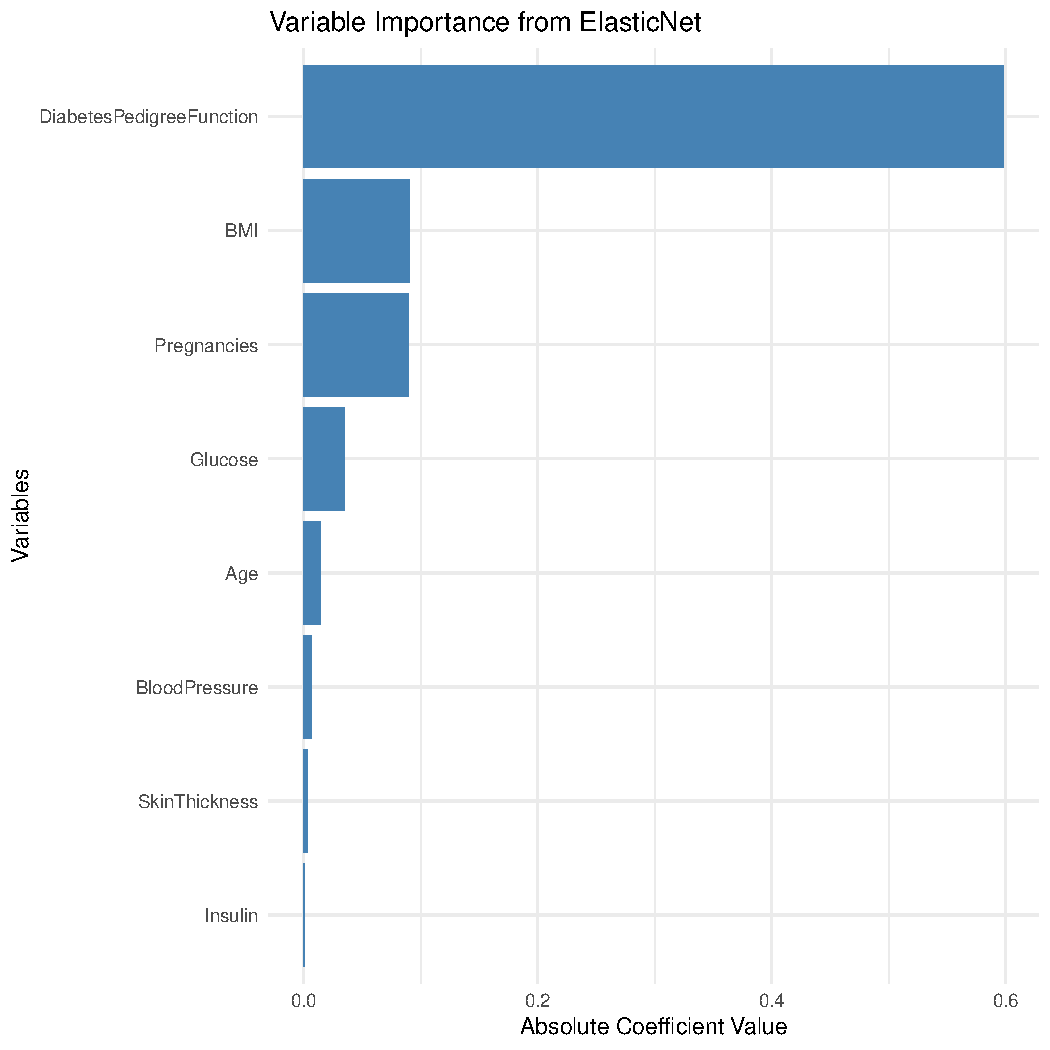
\includegraphics[width=0.7\columnwidth]{./Figures/logist/variable_importance_elasticnet.pdf}
\end{column}
\begin{column}{0.5\textwidth}
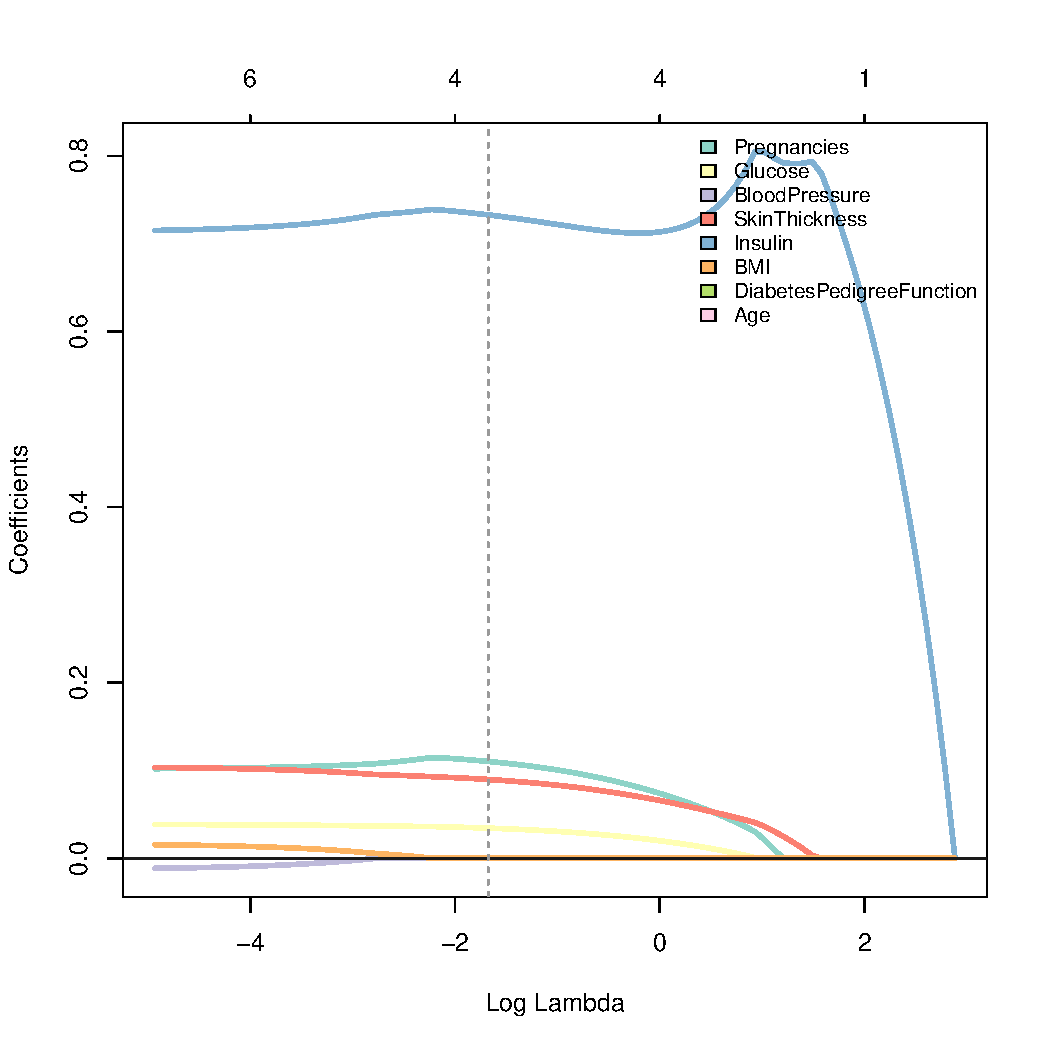
\includegraphics[width=0.85\columnwidth]{./Figures/logist/diabetes_adalasso.pdf}
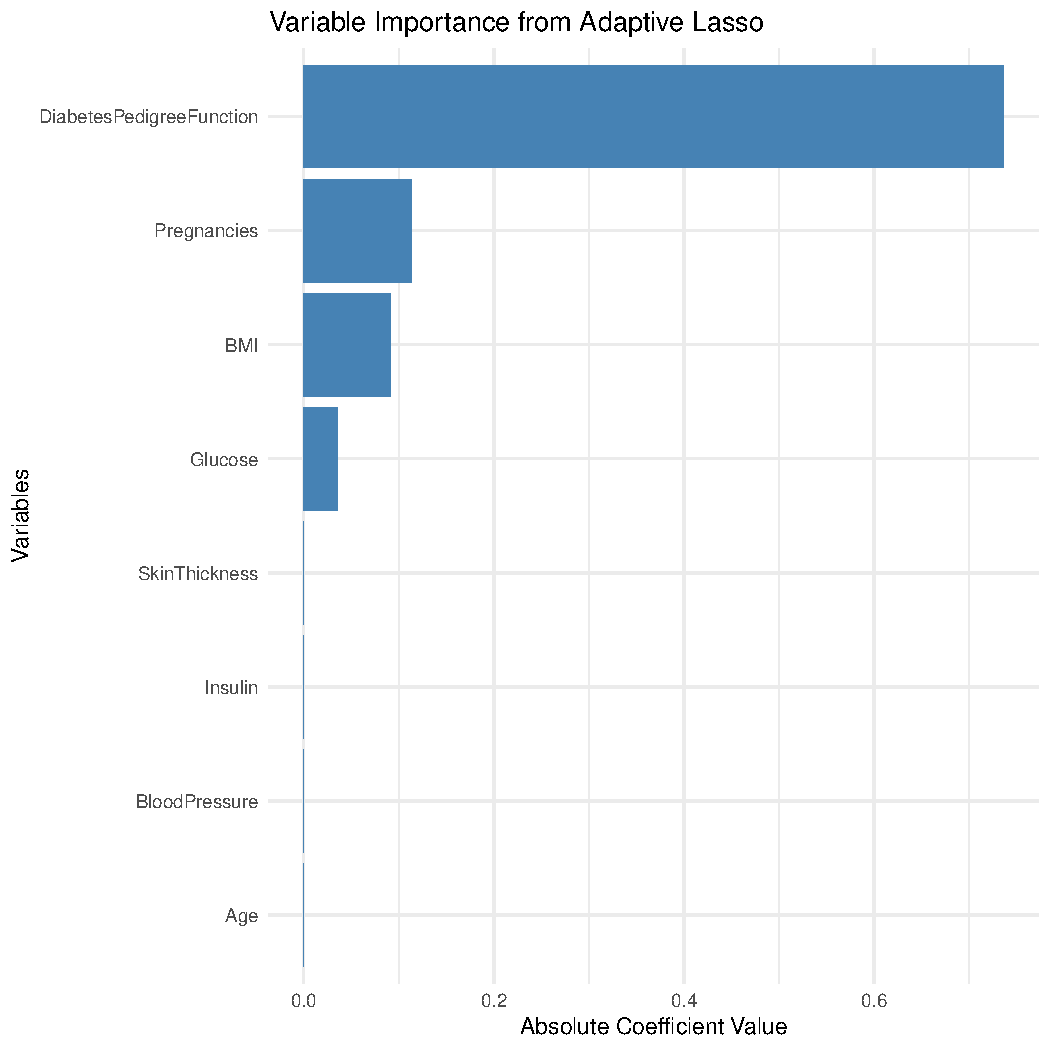
\includegraphics[width=0.7\columnwidth]{./Figures/logist/variable_importance_adalasso.pdf}
\end{column}
\end{columns}

\end{frame}

\begin{frame}{Results}
    \begin{table}
\sisetup{round-mode=places}
\resizebox{\textwidth}{!}{
\begin{tabular}{lS[round-precision=4]S[round-precision=4]S[round-precision=4]}
	Model & {Train score} & {Test score} & {\(\lambda\)} \\
	\midrule
	Lasso & 0.7714844 & 0.7695312 & 0.005678404 \\
	Ridge & 0.7695312 & 0.765625 & 0.02346324  \\
    ElasticNet & 0.7734375 & 0.7695312 & 0.008591009  \\
    AdaLasso & 0.7714844 & 0.7695312 & 0.005678404 \\
	\bottomrule
\end{tabular}}
\end{table}
\end{frame}
% !TeX spellcheck = en_GB

% ------------------------------- %
%% Random Forest Classifier %%
% ------------------------------- %

\begin{frame}{Random Forest for Classification}

{\small Package \texttt{\{randomForest\}}\vspace{-1.5ex}
\begin{itemize}\setlength{\itemsep}{-0.5ex}
	\item \lstinline|randomForest(formula, data=NULL, ntree=500, mtry=sqrt(p), importance=TRUE,|\texttt{\dots)}
	\item \lstinline|importance(x, type=NULL, class=NULL,|\texttt{\dots)}
    \item \lstinline|varImpPlot(x, sort=TRUE,|\texttt{\dots)}
    \item \texttt{x\$confusion}
    \item \texttt{x\$err.rate}
\end{itemize}}

{\texttt{x}} is a {\texttt{randomForest}} object;

{\texttt{ntree}} = number of trees grown;

{\texttt{p}} = number of predictors;

{\texttt{mtry}} = number of predictors sampled for splitting at each node.

\end{frame}

% ------------------------------- %

\begin{frame}{OOB Error}
\begin{columns}
\begin{column}{0.35\textwidth}

{\footnotesize \begin{itemize}
	\item $p$ = 8
	\item \texttt{mtry} = $\sqrt{p} \simeq 3$
	\item \texttt{ntree} = 500
	\item OOB estimate error rate: $24.41\%$
\end{itemize}}

\vspace{0.5cm}

\; Model selection:
{\footnotesize \begin{itemize}
	\item \texttt{ntree} = 111
	\item min OOB error rate = 0.2343
\end{itemize}}

\end{column}
\begin{column}{0.75\textwidth}
\begin{figure}
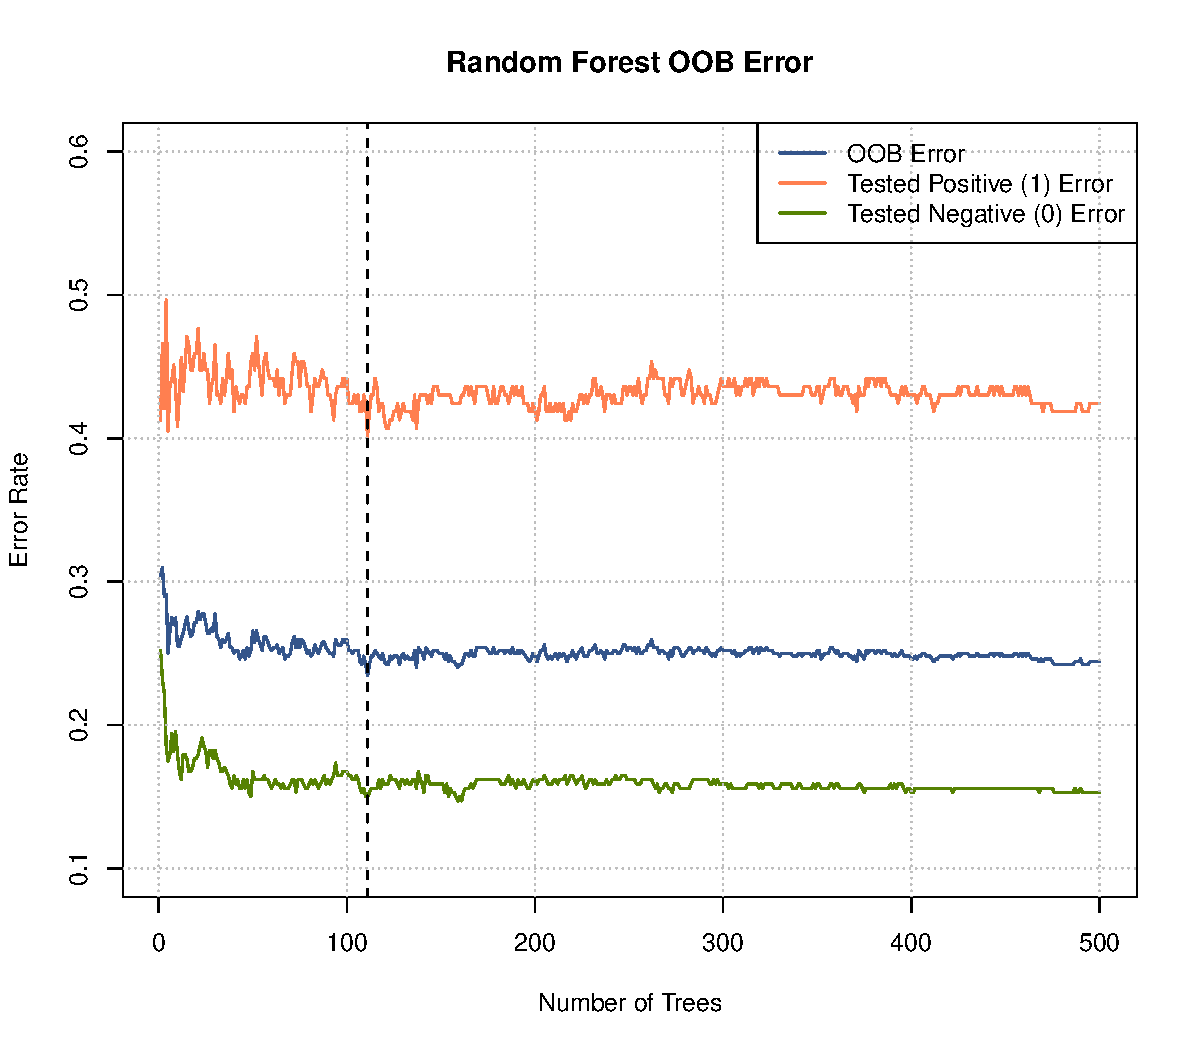
\includegraphics[width=1.05\columnwidth]{./Figures/forest/diabete_forest_error3.pdf}
\end{figure}
\end{column}
\end{columns}
\end{frame}

% ------------------------------- %

\begin{frame}{OOB Error}

\begin{columns}
\begin{column}{0.35\textwidth}
{\footnotesize \begin{itemize}
	\item $p$ = 8
	\item \texttt{mtry} = 4 
	\item \texttt{ntree} = 500
	\item OOB estimate error rate: $25\%$
\end{itemize}}

\vspace{0.5cm}

\; Model selection:
{\footnotesize \begin{itemize}
	\item \texttt{ntree} = 136
	\item min OOB error rate = 0.2226
\end{itemize}}

\end{column}
\begin{column}{0.75\textwidth}
\begin{figure}
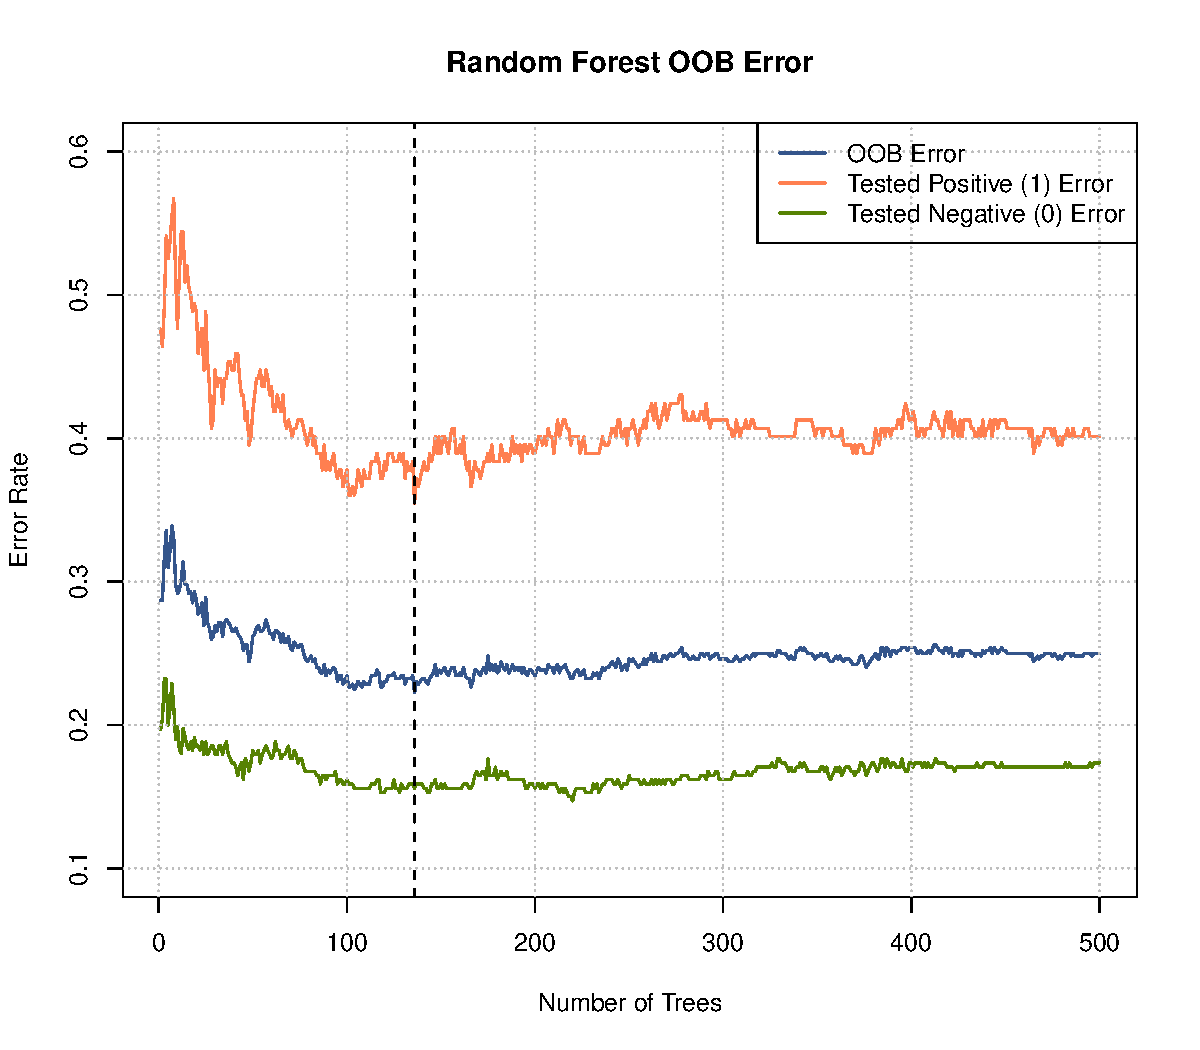
\includegraphics[width=1.05\columnwidth]{./Figures/forest/diabete_forest_error4.pdf}
\end{figure}
\end{column}
\end{columns}

\end{frame}

% ------------------------------- %

\begin{frame}%{Variable Importance}

\begin{figure}
\hspace*{-1.5em}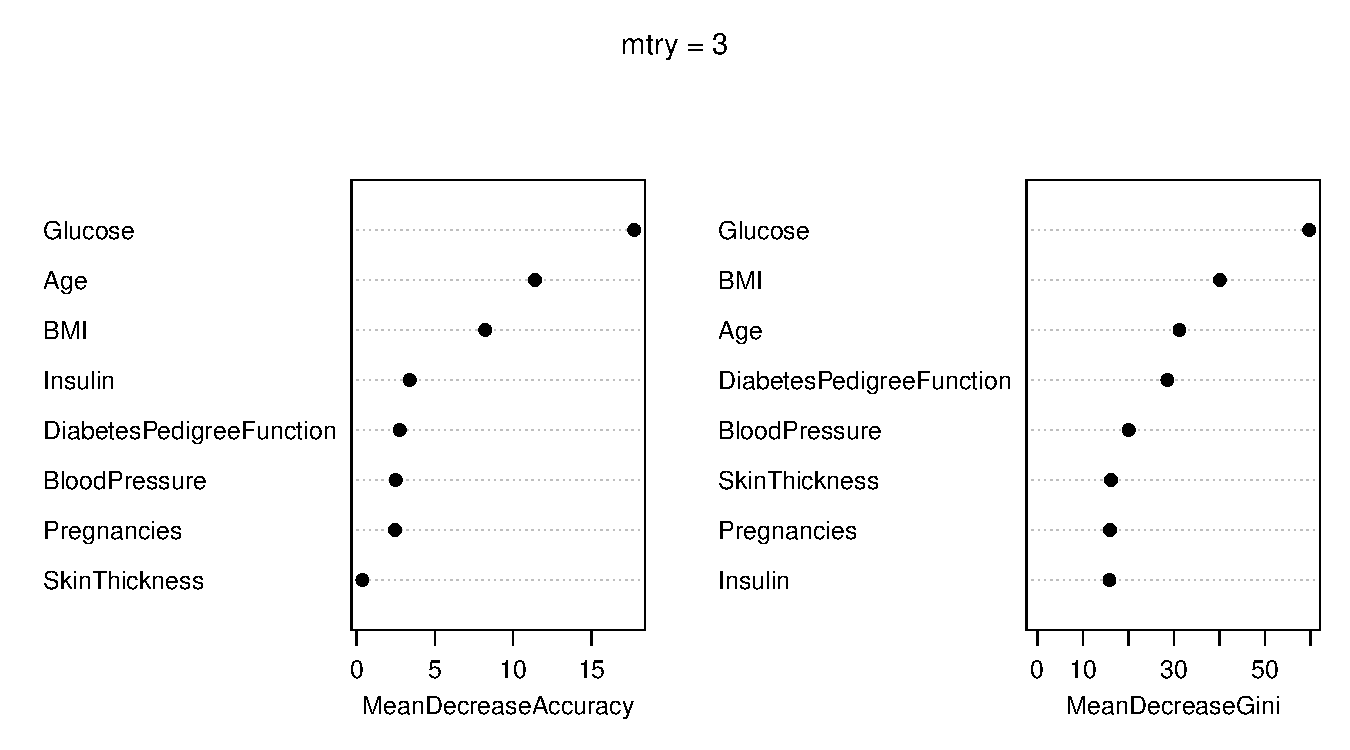
\includegraphics[width=0.78\textwidth]{./Figures/forest/diabete_var_imp3.pdf}
\hspace*{-1.5em}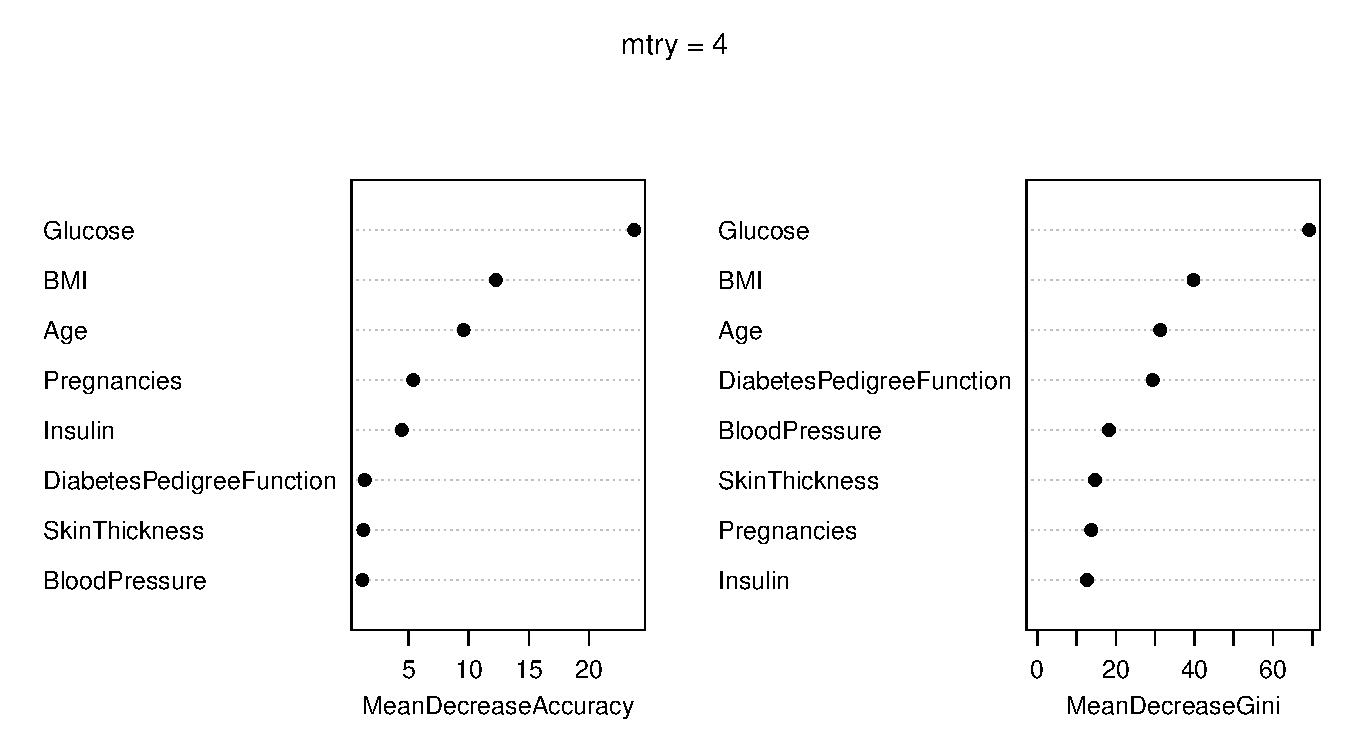
\includegraphics[width=0.78\textwidth]{./Figures/forest/diabete_var_imp4.pdf}
\end{figure}
\end{frame}

% ------------------------------- %

% !TeX spellcheck = en_GB

% ------------------------------- %
%% Introduction, AdaBoost classifier %%
% ------------------------------- %

%\begin{frame}{The idea behind AdaBoost \,\,i}
%What are we predicting?
%
%$\mathcal{Y}\in\set{-1,1}$
%
%Weak learner, base classifier
%
%\begin{figure}
%%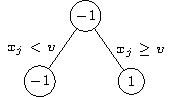
\includegraphics[width=0.3\textwidth,page=1]{./Figures/drawings/drawings.pdf}
%\begin{tikzpicture}[]
%	\tikzset{help lines/.append style=pink}
%	%	\draw [help lines] (-2,-2) grid (2,1);
%	
%	\node[treenode] (root) at (0,0) {$-1$};
%	\node[treenode] (root-l) at (-125:1.35) {$-1$};
%	\node[treenode] (root-r) at (-55:1.35) {$1$};
%	
%	\draw[-] (root) -- node[font=\scriptsize,left] {$x_j<v$} (root-l);
%	\draw[-] (root) -- node[font=\scriptsize,right] {$x_j\geq v$} (root-r);
%\end{tikzpicture}
%\end{figure}
%
%\end{frame}

% ------------------------------- %

%\begin{frame}{The idea behind AdaBoost \,\,i}
%%
%\begin{columns}[T]
%\begin{column}{0.48\textwidth}
%\begin{figure}
%\centering
%\begin{tikzpicture}
%	%draw,ellipse,fill=red!20,minimum height=2em,text centered,font=\sffamily\small
%	\tikzset{help lines/.append style=pink}
%	%\draw [help lines] (-2,-8) grid (3,1);
%
%	\begingroup\linespread{0.95}
%	\node[cloud] (m1) at (0,0) {training data};
%	\node[cloud] (m2) at (0,-1.5) {weighted data};
%	\node[cloud] (M) at (0,-4.5) {weighted data};
%	\endgroup
%	\draw[-latex] (m1) to (m2);
%	\draw[-,dotted,very thick] ($(m2.south) + (0,-0.15)$) to ($(M.north) + (0,+0.15)$);
%	
%	\node (G1) at (2.3,0) {$G_1(x)$};
%	\node (G2) at (2.3,-1.5) {$G_2(x)$};
%	\node (GM) at (2.3,-4.5) {$G_M(x)$};
%	\draw[-stealth] ($(m1.east) + (0.15,0)$) to (G1);
%	\draw[-stealth] ($(m2.east) + (0.15,0)$) to (G2);
%%	\draw[-,dotted] (G2) to (GM);
%	\draw[-stealth] ($(M.east) + (0.15,0)$) to (GM);
%
%%	\node[rectangle,fill=pink!80] (G) at (1.5,-6) {$G(x)=\sign\Bigl(\sum_{m=1}^M\beta_mG_m(x)\Bigr)$};
%	\node[rectangle,fill=mLightGreen!20,font=\large] (G) at (1.6,-6.2) {$G(x)=\sign\Bigl(\lambda\sum_{m=1}^M\alpha_mG_m(x)\Bigr)$};
%%	\draw[-stealth] (GM) to (G);
%\end{tikzpicture}
%\end{figure}
%\end{column}
%\begin{column}{0.48\textwidth}
%\vspace{0.6em}
%Journey to the final classifier:
%{\small\begin{itemize}
%	\setlength{\itemsep}{-0.8ex}
%	\item Linear combination of \alert{weak learners}
%	\item Adaptively build up complexity
%	\item Early stopping to achieve regularization
%	\item \alert{Re-weighting} of training data  % permette all'algoritmo di concentrarsi sugli esempi più difficili da classificare, quindi di questi esempi viene aumentato il peso
%\end{itemize}}
%\vspace{0.8em}
%%Loss function:
%%\[L(y,f(x))=\exp(-yf(x))\]
%Misclassification rate:\vspace{-1ex}
%\[
%\overline{\text{err}}=\frac{1}{N}\sum_{i=1}^N\mathbb{I}(y_i\neq G(x_i))
%\]
%%\begin{figure}
%%\centering
%%\begin{tikzpicture}
%%	\begin{axis}[xlabel=$yf(x)$,ylabel={$L$},axis lines=middle,enlargelimits,width=0.9\textwidth]
%%		\addplot[samples=200,blue,smooth] {exp(-x)};
%%		%\addplot[dashed] {1};
%%%		\addplot [black, mark=-, nodes near coords=$\log(2)$, font={\scriptsize}, every node near coord/.style={anchor=180}] coordinates {(0,{ln(2)})};
%%	\end{axis}
%%\end{tikzpicture}
%%\end{figure}
%\end{column}
%\end{columns}
%
%\end{frame}



\begin{frame}{The idea behind AdaBoost (Discrete AdaBoost)}
%
\begin{columns}[T]
\begin{column}{0.48\textwidth}
\begin{figure}
\centering
\begin{tikzpicture}
	%draw,ellipse,fill=red!20,minimum height=2em,text centered,font=\sffamily\small
	\tikzset{help lines/.append style=pink}
	%\draw [help lines] (-2,-8) grid (3,1);
	
	\begingroup\linespread{0.95}
	\node[cloud] (m1) at (0,0) {training data};
	\node[cloud] (m2) at (0,-1.5) {weighted data};
	\node[cloud] (M) at (0,-4.5) {weighted data};
	\endgroup
	\draw[-latex] (m1) to (m2);
	\draw[-,dotted,very thick] ($(m2.south) + (0,-0.15)$) to ($(M.north) + (0,+0.15)$);
	
	\node (G1) at (2.3,0) {$G_1(x)$};
	\node (G2) at (2.3,-1.5) {$G_2(x)$};
	\node (GM) at (2.3,-4.5) {$G_M(x)$};
	\draw[-stealth] ($(m1.east) + (0.15,0)$) to (G1);
	\draw[-stealth] ($(m2.east) + (0.15,0)$) to (G2);
	%	\draw[-,dotted] (G2) to (GM);
	\draw[-stealth] ($(M.east) + (0.15,0)$) to (GM);
	
	%	\node[rectangle,fill=pink!80] (G) at (1.5,-6) {$G(x)=\sign\Bigl(\sum_{m=1}^M\beta_mG_m(x)\Bigr)$};
	\node[rectangle,fill=mLightGreen!20,font=\large] (G) at (1.6,-6.2) {$G(x)=\sign\Bigl(\sum_{m=1}^M\alpha_mG_m(x)\Bigr)$};
	%	\draw[-stealth] (GM) to (G);
\end{tikzpicture}
\end{figure}
\end{column}
\begin{column}{0.48\textwidth}
\vspace{1em}
Encoding $\mathcal{Y}\in\set{-1,1}$

Base classifier $G_m(x)$ (CART)
\begin{figure}
%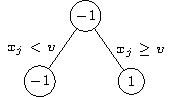
\includegraphics[width=0.3\textwidth,page=1]{./Figures/drawings/drawings.pdf}
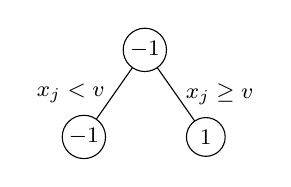
\begin{tikzpicture}[]
	\tikzset{help lines/.append style=pink}
	%	\draw [help lines] (-2,-2) grid (2,1);
	
	\node[treenode] (root) at (0,0) {$-1$};
	\node[treenode] (root-l) at (-125:1.35) {$-1$};
	\node[treenode] (root-r) at (-55:1.35) {$1$};
	
	\draw[-] (root) -- node[font=\footnotesize,left] {$x_j<v$} (root-l);
	\draw[-] (root) -- node[font=\footnotesize,right] {$x_j\geq v$} (root-r);
\end{tikzpicture}
\end{figure}

\vspace{1em}
Misclassification rate:\vspace{-1ex}
\[
\overline{\text{err}}=\frac{1}{N}\sum_{i=1}^N\mathbb{I}(y_i\neq G(x_i))
\]

\vspace{-0.7cm}\hspace{-0.25ex}\begin{tikzpicture}
	\tikzset{help lines/.append style=pink}
%	\draw [help lines] (-2,-1) grid (2,1); \node[draw,circle] at (0,0) {};

	\draw[-stealth,bend right=35,thick] (-2,0.3) to (1.7,1.6);
\end{tikzpicture}

\end{column}
\end{columns}

\end{frame}

% ------------------------------- %

\begin{frame}{AdaBoost as an additive model and stochastic setting}
% modello additivo perché in ogni albero c'è soltanto una variabile
\begin{columns}[T]
\begin{column}{0.48\textwidth}
\begin{figure}
\centering
\vspace*{-0.5em}\begin{tikzpicture}
	%draw,ellipse,fill=red!20,minimum height=2em,text centered,font=\sffamily\small
	\tikzset{help lines/.append style=pink}
	%	\draw [help lines] (-2,-8) grid (3,1); \node[draw,circle,red] at (0,0) {};
	
	\node[cloud2] (m1) at (0,0) {$w^{(1)}, \pi_1$};
	\node[cloud2] (m2) at (0,-1.25) {$w^{(2)}, \pi_2$};
	\node[cloud2] (M) at (0,-4.5) {$w^{(M)}, \pi_M$};
	\draw[-latex] (m1) to (m2);
	\draw[-,dotted,very thick] ($(m2.south) + (0,-0.15)$) to ($(M.north) + (0,+0.15)$);
	
	\node (G1) at (2.3,0) {$G_1, f_1$};
	\node (G2) at (2.3,-1.25) {$G_2, f_2$};
	\node (GM) at (2.3,-4.5) {$G_M, f_M$};
	\draw[-stealth] ($(m1.east) + (0.15,0)$) to (G1);
	\draw[-stealth] ($(m2.east) + (0.15,0)$) to (G2);
	%	\draw[-,dotted] (G2) to (GM);
	\draw[-stealth] ($(M.east) + (0.15,0)$) to (GM);
	
	%	\node[rectangle,fill=pink!80] (G) at (1.5,-6) {$G(x)=\sign\Bigl(\sum_{m=1}^M\beta_mG_m(x)\Bigr)$};
%	\node[rectangle,fill=teal!20,font=\large,right] (f) at (-1,-5.55) {$L(y,f(x))=\exp(-yf(x))$};
	\node[rectangle,fill=teal!20,font=\large,right] (G) at (-1,-5.7) {$f_m(x)=f_{m-1}(x)+\lambda\alpha_mG_m(x)$};
	\node[rectangle,fill=mLightGreen!20,font=\large,right] (L) at (-1,-6.5) {$G(x)=\sign(f_M(x))$};
	%	\draw[-stealth] (GM) to (G);
	
	\begingroup\linespread{0.9}
	\node[font=\footnotesize,text width=4em,centered,text centered,inner sep=0pt] (pi) at (2.8,-2.6) {dataset random subsample};
	\endgroup
	\draw[-stealth] (pi) to ($(m2.east) + (-0.25,-0.1)$);
\end{tikzpicture}
\end{figure}
\end{column}
\begin{column}{0.48\textwidth}
\vspace{0.7em}
Journey to the final classifier:
{\footnotesize\begin{itemize}
	\setlength{\itemsep}{-0.8ex}
	\item Linear combination of \alert{weak learners} (additive model)
	\item Adaptively build up complexity, through a prediction function
	\item Regularization with early stopping and shrinkage
	\item \alert{Re-weighting} of a bootstrapped fraction of the training data  % permette all'algoritmo di concentrarsi sugli esempi più difficili da classificare, quindi di questi esempi viene aumentato il peso
\end{itemize}}
%$f_m(x)$ prediction function

%$\lambda$ shrinkage coefficient


\vspace{0.8em}
Exponential loss function:\vspace{-1ex}
\[L(y,f(x))=\exp(-yf(x))\]
%\begin{figure}
%\centering
%\begin{tikzpicture}
%	\begin{axis}[xlabel=$yf(x)$,ylabel={$L$},axis lines=middle,enlargelimits,width=1.2\textwidth]
%		\addplot[samples=200,blue,smooth] {exp(-x)};
%		%\addplot[dashed] {1};
%%		\addplot [black, mark=-, nodes near coords=$\log(2)$, font={\scriptsize}, every node near coord/.style={anchor=180}] coordinates {(0,{ln(2)})};
%	\end{axis}
%\end{tikzpicture}
%\end{figure}
\end{column}
\end{columns}

\end{frame}

% ------------------------------- %

\begin{frame}{AdaBoost in practice}
\vspace*{-2.5em}\lstinline|ada::ada(formula, data, loss="exponential", type="discrete", iter, nu=0.01, bag.frac)|\bigskip\smallskip

\begin{columns}[T]
\begin{column}{0.5\textwidth}
Function \texttt{ada} arguments:\vspace{-1ex}
{\small\begin{itemize}
	\setlength{\itemsep}{-0.8ex}
	\item \texttt{loss}: boosting loss function
	\item \texttt{type}: AdaBoost version
	\item \texttt{iter}: boosting rounds
	\item \texttt{nu}: shrinkage coefficient $\lambda$
	\item \texttt{bag.frac}: in-bag fraction \numlist{1;0.5}
\end{itemize}}
\end{column}
\begin{column}{0.5\textwidth}
%Journey to the final classifier:
%{\small\begin{itemize}
%\setlength{\itemsep}{-0.8ex}
%\item Linear combination of \alert{weak learners} (additive model)
%\item Adaptively build up complexity, through a prediction function
%\item Regularization with early stopping and shrinkage
%\item \alert{Re-weighting} of a subsample of the training data  % permette all'algoritmo di concentrarsi sugli esempi più difficili da classificare, quindi di questi esempi viene aumentato il peso
%\end{itemize}}
\begin{figure}
% quando è classificato correttamente y e f(x) avranno segno concorde, la funzione andrà a 0
% quando il label non è corretto, il segno discorde manda la funzione a infinito
\begin{tikzpicture}
\begin{axis}[xlabel=$yf(x)$,ylabel={$L(y,f(x))$},axis lines=middle,enlargelimits,width=1.1\textwidth,tick label style={font=\scriptsize}]
	\addplot[samples=200,blue,smooth,thick] {exp(-x)};
	%\addplot[dashed] {1};
\end{axis}
\end{tikzpicture}
\end{figure}
\end{column}
\end{columns}

\end{frame}




%\begin{frame}{coide}
%
%{\footnotesize Package \texttt{\{randomForest\}}\vspace{-1ex}
%\begin{itemize}\setlength{\itemsep}{-0.5ex}
%	\item \texttt{randomForest(formula, data={\color{blue}NULL}, ntree={\color{red}500}, mtry={\color{blue}sqrt}(p), importance={\color{red}TRUE}, \dots)}
%	\item \lstinline|randomForest(formula, data=NULL, ntree=500, mtry=sqrt(p), importance=TRUE)|
%	\item \texttt{importance(x, type={\color{blue}NULL}, class={\color{blue}NULL}, \dots)}
%	\item \texttt{varImpPlot(x, sort={\color{red}TRUE}, \dots)}
%	\item \texttt{rf.model\$confusion}
%	\item \texttt{rf.model\$err.rate}
%\end{itemize}}
%\end{frame}


% !TeX spellcheck = en_GB

% ------------------------------- %
%% Dataset, fitting, results %%
% ------------------------------- %

\begin{frame}{Fit AdaBoost}

%\hspace{-1em}
%\begin{figure}
%\subfloat{\includegraphics[width=0.5\paperwidth]{../r/plots/cv-adaboost.pdf}}
%\subfloat{\includegraphics[width=0.5\paperwidth]{../r/plots/adaboost-varimp.pdf}}
%\end{figure}

%$M_{\text{max}}=1000$, $\lambda=0.1$, $\pi=0.5$

%\texttt{ada::ada(<\emph{data}>, loss="exponential", type="discrete", nu=0.1, iter=1000, bag.frac=0.5)}

\begin{columns}[T]
\hspace{-2.3em}\begin{column}{0.515\textwidth}
	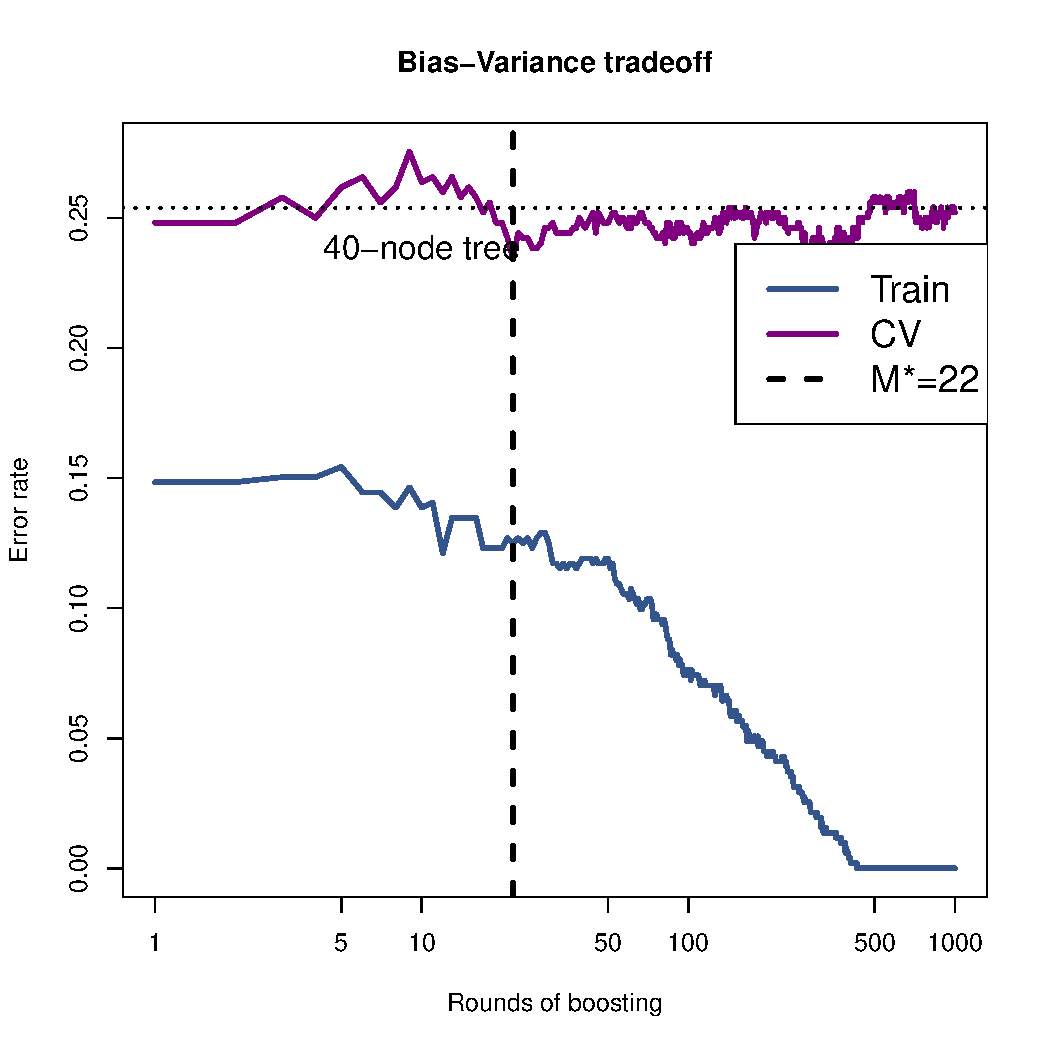
\includegraphics[width=1.21\columnwidth]{../r/plots/cv-adaboost-diab.pdf}
\end{column}
\hspace{-1.3ex}\begin{column}{0.515\textwidth}
	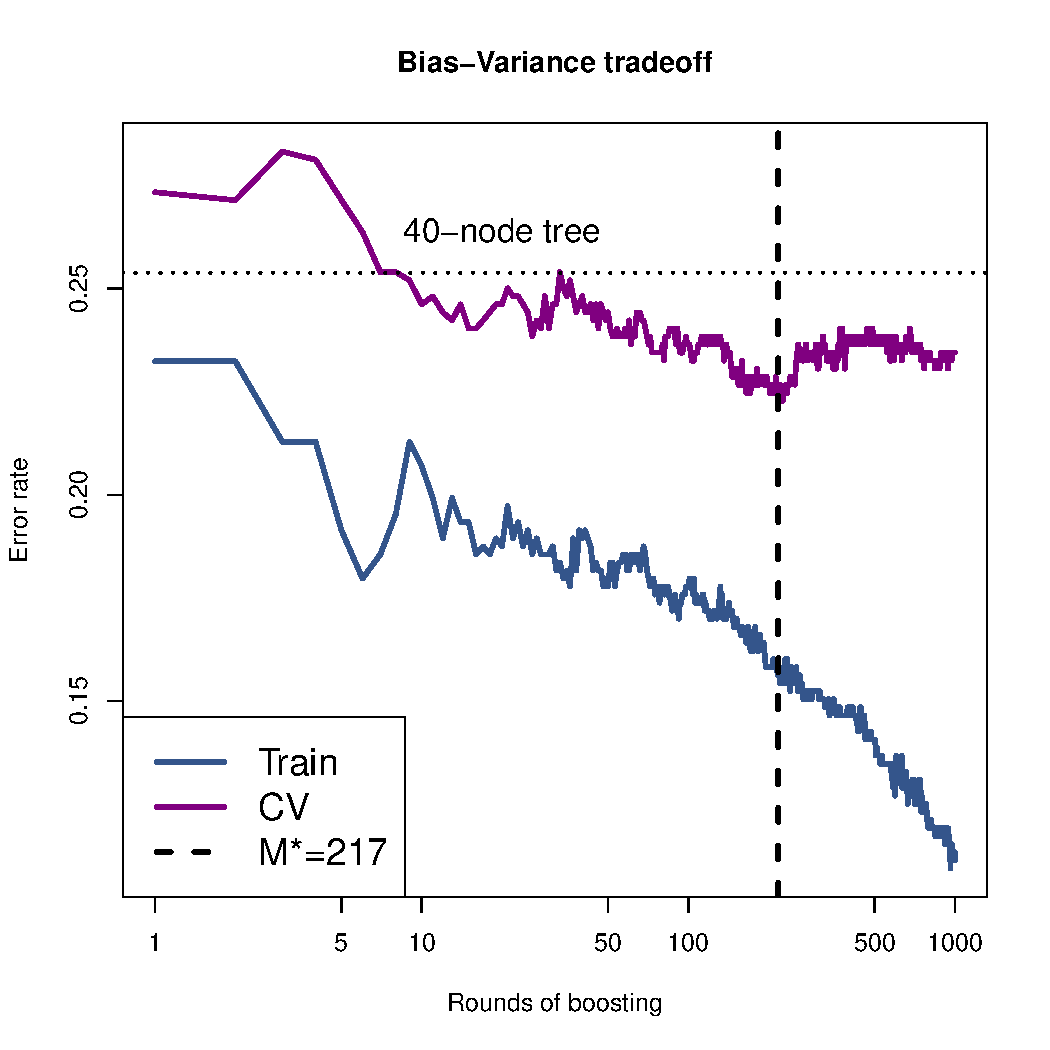
\includegraphics[width=1.21\columnwidth]{../r/plots/cv-adaboost-st-diab.pdf}
\end{column}
\end{columns}

\end{frame}

% col bagging ha bisogno di maggiori iterazioni prima di arricare all'overfitting (anche se nel boosting non si verifica effettivamente, è solo teorico)

%\begin{frame}{Fit AdaBoost (apple quality)}
%
%\begin{columns}[T]
%\hspace{-2.3em}\begin{column}{0.515\textwidth}
%	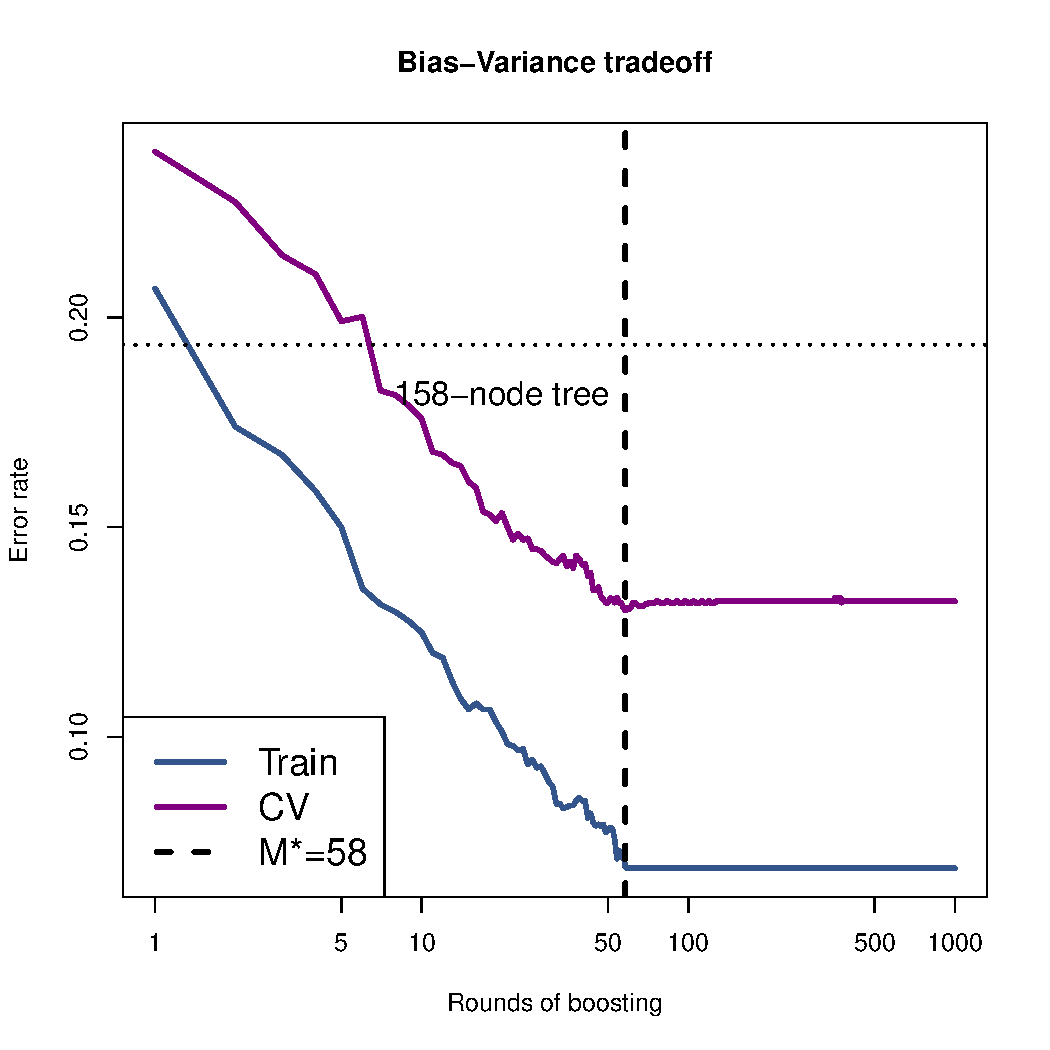
\includegraphics[width=1.21\columnwidth]{../r/plots/cv-adaboost-apple.pdf}
%\end{column}
%\hspace{-1.3ex}\begin{column}{0.515\textwidth}
%	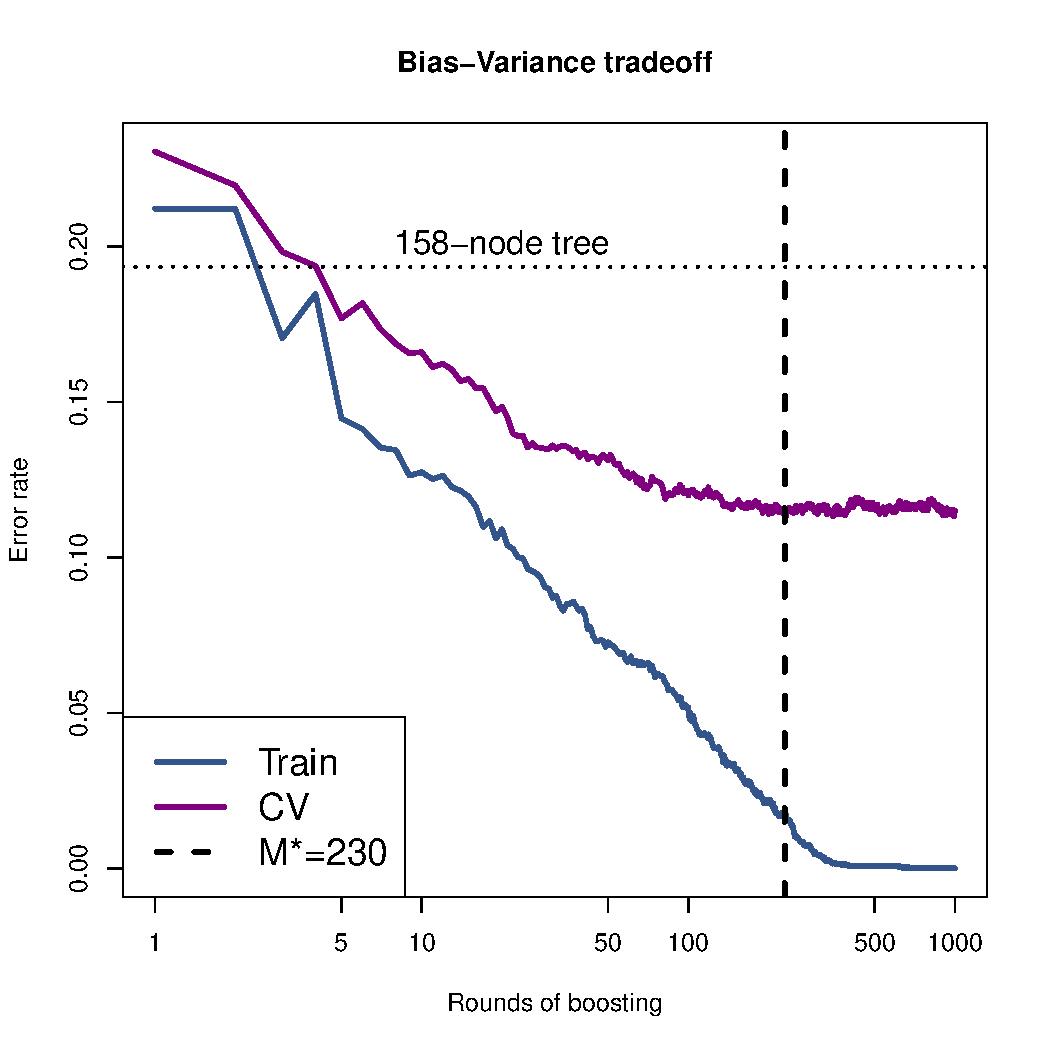
\includegraphics[width=1.21\columnwidth]{../r/plots/cv-adaboost-st-apple.pdf}
%\end{column}
%\end{columns}
%
%\end{frame}

% ------------------------------- %

%\begin{frame}{AdaBoost stochastic setting}

% a sinistra qualcosa di teoria (tipo il journey to the final classifier)
% a destra il bias-variance

%\vspace*{-0.5em}\begin{columns}[T]
%\begin{column}{0.48\textwidth}
%\begin{figure}
%\hspace{-2em}\begin{tikzpicture}
%	%draw,ellipse,fill=red!20,minimum height=2em,text centered,font=\sffamily\small
%	\tikzset{help lines/.append style=pink}
%%	\draw [help lines] (-2,-8) grid (3,1); \node[draw,circle,red] at (0,0) {};
%	
%	\node[cloud2] (m1) at (0,0) {$w^{(1)}, \pi_1$};
%	\node[cloud2] (m2) at (0,-1.25) {$w^{(2)}, \pi_2$};
%	\node[cloud2] (M) at (0,-4.5) {$w^{(M)}, \pi_M$};
%	\draw[-latex] (m1) to (m2);
%	\draw[-,dotted,very thick] ($(m2.south) + (0,-0.15)$) to ($(M.north) + (0,+0.15)$);
%	
%	\node (G1) at (2.3,0) {$G_1, f_1$};
%	\node (G2) at (2.3,-1.25) {$G_2, f_2$};
%	\node (GM) at (2.3,-4.5) {$G_M, f_M$};
%	\draw[-stealth] ($(m1.east) + (0.15,0)$) to (G1);
%	\draw[-stealth] ($(m2.east) + (0.15,0)$) to (G2);
%	%	\draw[-,dotted] (G2) to (GM);
%	\draw[-stealth] ($(M.east) + (0.15,0)$) to (GM);
%	
%	%	\node[rectangle,fill=pink!80] (G) at (1.5,-6) {$G(x)=\sign\Bigl(\sum_{m=1}^M\beta_mG_m(x)\Bigr)$};
%	\node[rectangle,fill=teal!20,font=\large,right] (f) at (-1,-5.55) {$L(y,f(x))=\exp(-yf(x))$};
%	\node[rectangle,fill=red!20,font=\large,right] (G) at (-1,-6.3) {$f_m(x)=f_{m-1}(x)+\lambda\alpha_mG_m(x)$};
%	\node[rectangle,fill=mLightGreen!20,font=\large,right] (L) at (-1,-7.05) {$G(x)=\sign(f_M(x))$};
%	%	\draw[-stealth] (GM) to (G);
%
%	\begingroup\linespread{0.9}
%	\node[font=\footnotesize,text width=4em,centered,text centered,inner sep=0pt] (pi) at (2.8,-2.6) {dataset random subsample};
%	\endgroup
%	\draw[-latex] (pi) to ($(m2.east) + (-0.25,-0.1)$);
%\end{tikzpicture}
%\end{figure}
%\end{column}
%\begin{column}{0.48\textwidth}
%\begin{figure}
%	\hspace*{-1.8em}\includegraphics[width=1.3\columnwidth]{../r/plots/cv-adaboost-st.pdf}
%\end{figure}
%$\pi=0.7$, $\lambda=0.1$
%% il learning rate basso viene compensato dal M* alto
%\end{column}
%\end{columns}
%
%\end{frame}



\begin{frame}{Variable importance}

\begin{columns}[T]
\hspace{-2.5em}\begin{column}{0.515\textwidth}
	% boosting setting
	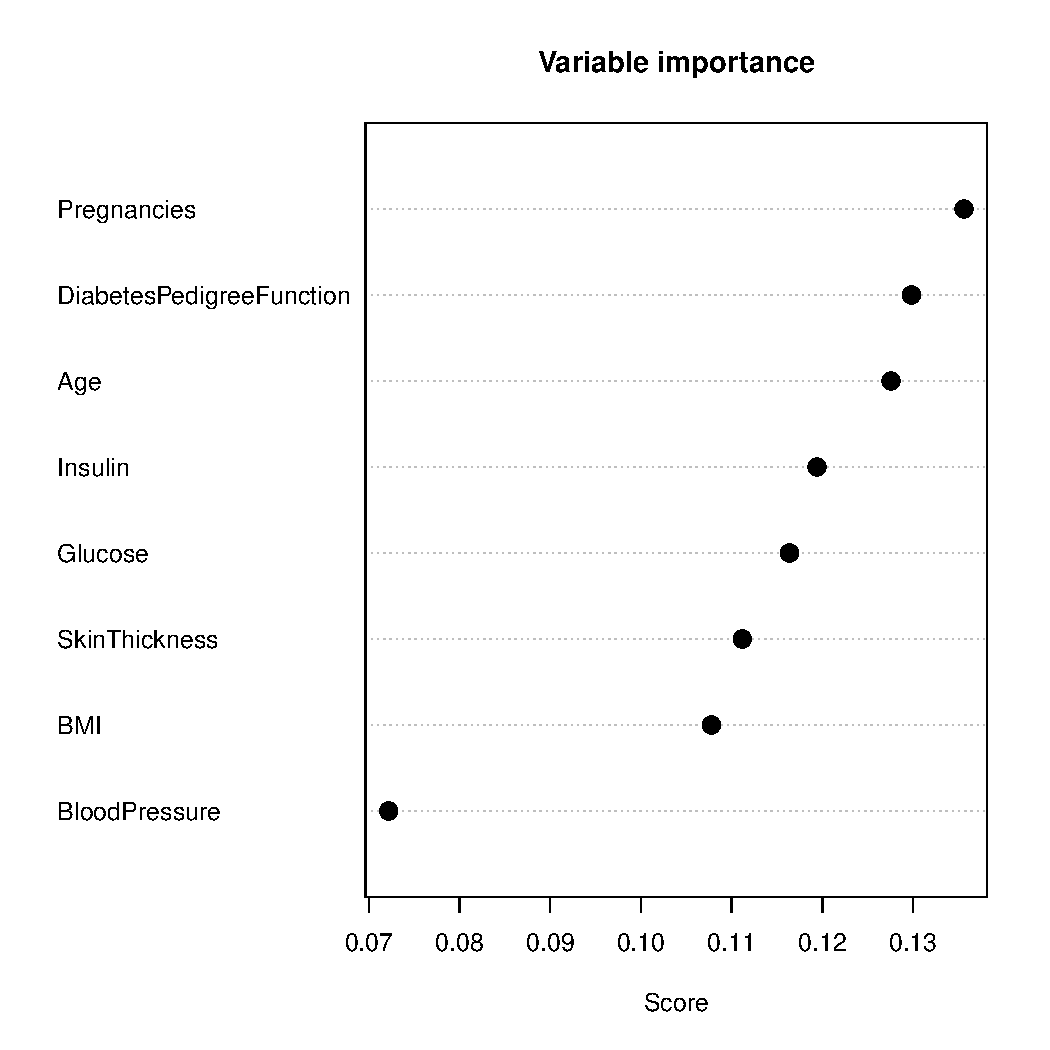
\includegraphics[width=1.21\columnwidth]{../r/plots/vip-adaboost-diab.pdf}
\end{column}
\hspace{-1.3ex}\begin{column}{0.515\textwidth}
	% stochastic setting
	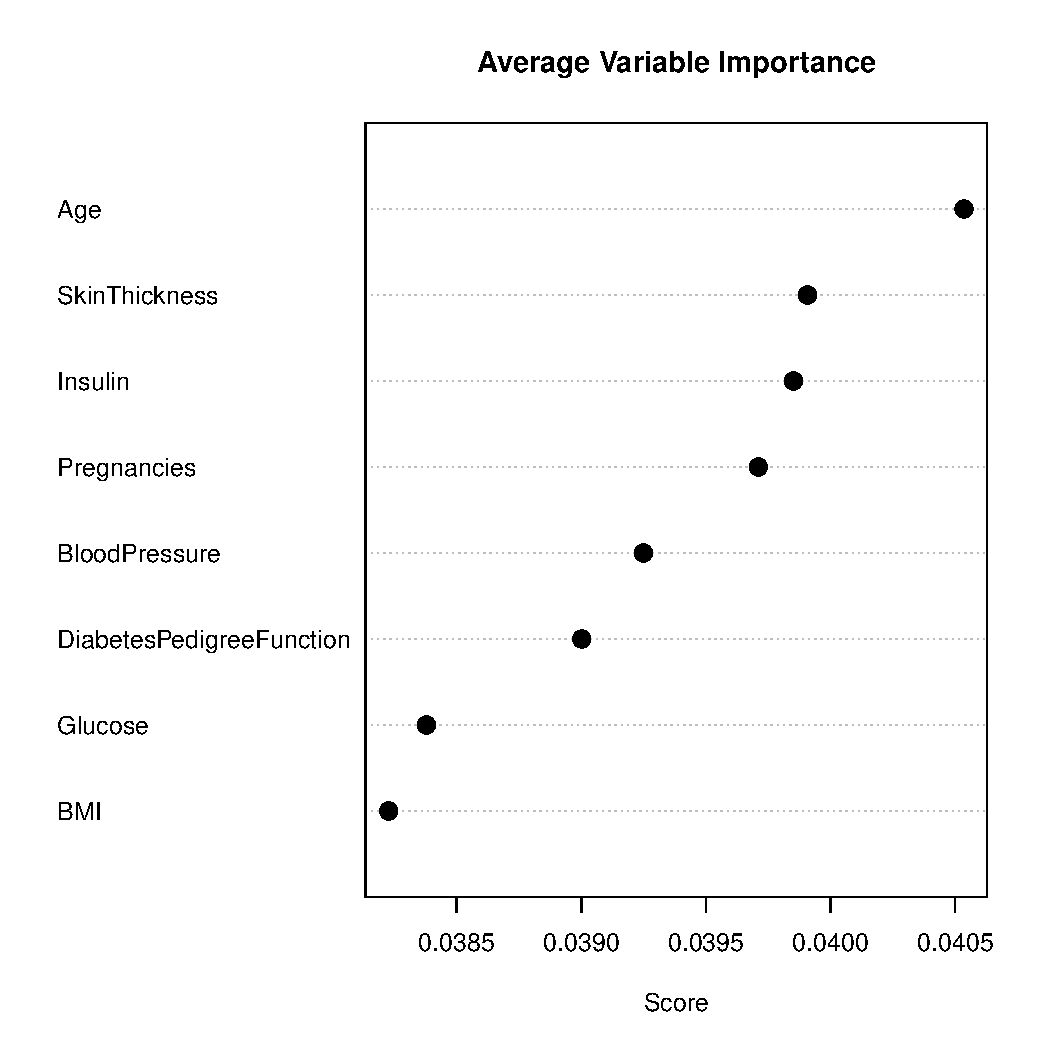
\includegraphics[width=1.21\columnwidth]{../r/plots/vip-adaboost-st1-diab.pdf}
\end{column}
\end{columns}

\end{frame}



%\begin{frame}{Variable importance (apple quality)}
%
%\begin{columns}[T]
%\hspace{-2.5em}\begin{column}{0.515\textwidth}
%	% boosting setting
%	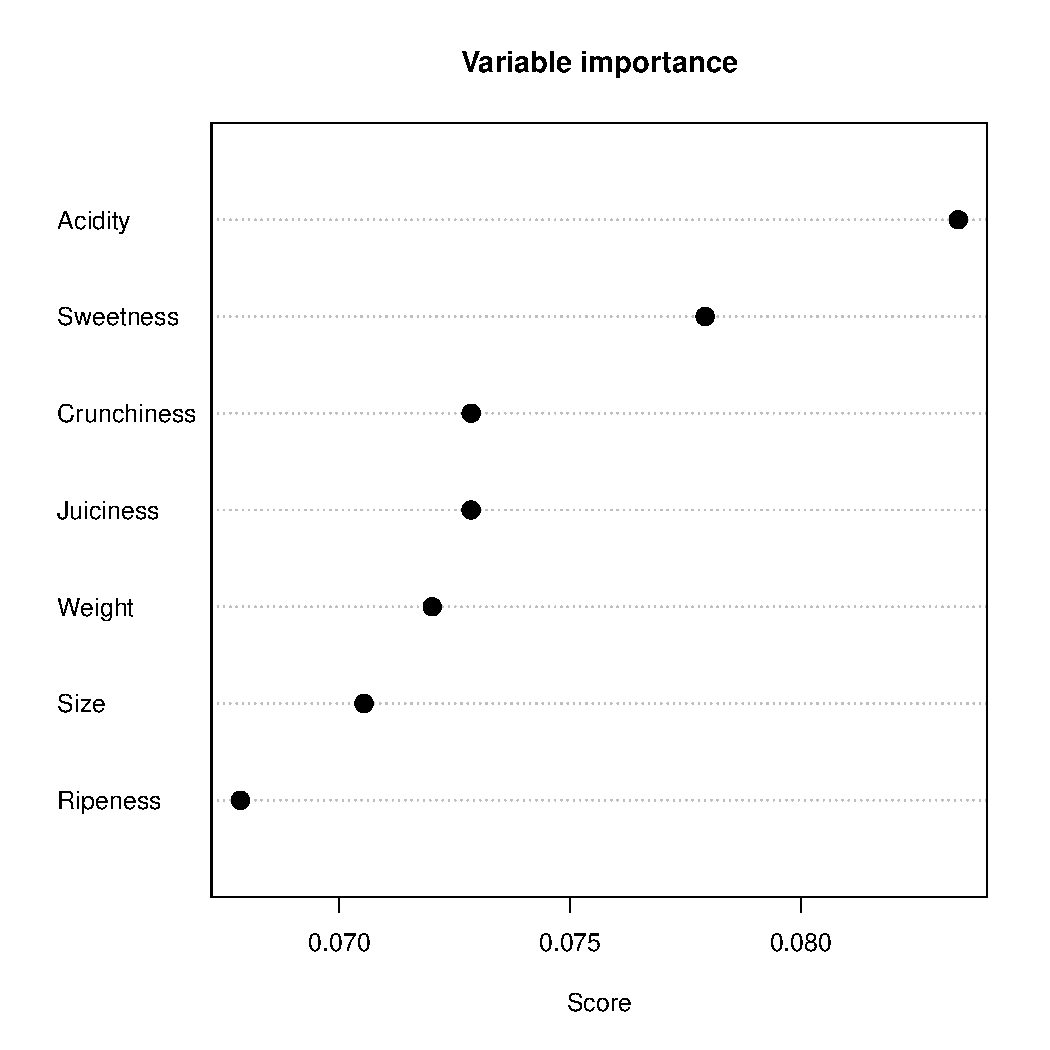
\includegraphics[width=1.21\columnwidth]{../r/plots/vip-adaboost-apple.pdf}
%\end{column}
%\hspace{-1.3ex}\begin{column}{0.515\textwidth}
%	% stochastic setting
%	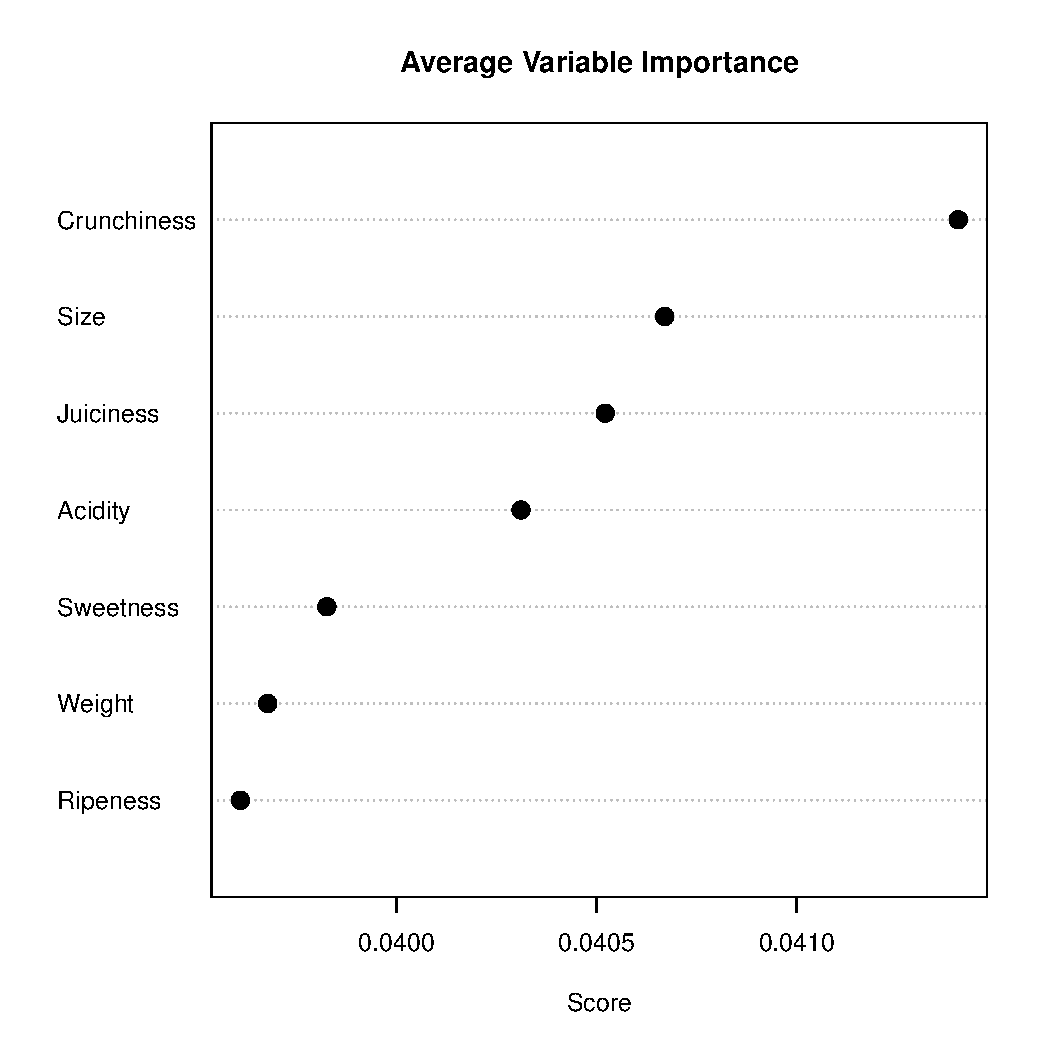
\includegraphics[width=1.21\columnwidth]{../r/plots/vip-adaboost-st1-apple.pdf}
%\end{column}
%\end{columns}
%
%\end{frame}



%\begin{frame}%{All models variable importance}
%
%% change plot title with model name
%% remove xlab (from R or just trim it)
%
%\vspace*{-0.5em}
%\begin{columns}[T]
%\hspace{1em}\begin{column}{0.515\textwidth}
%	% boosting setting
%	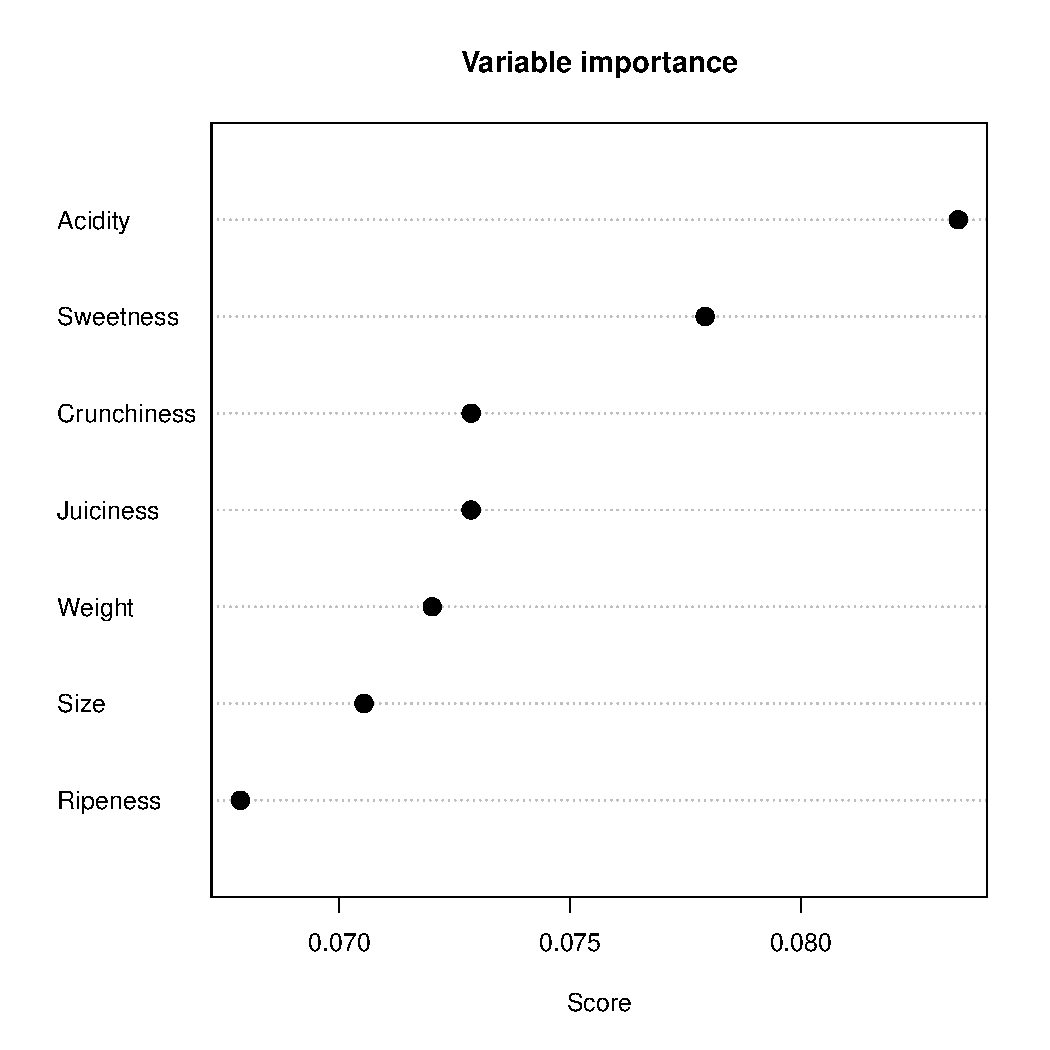
\includegraphics[width=0.9\columnwidth]{../r/plots/vip-adaboost-apple.pdf}\vspace{-1em}
%	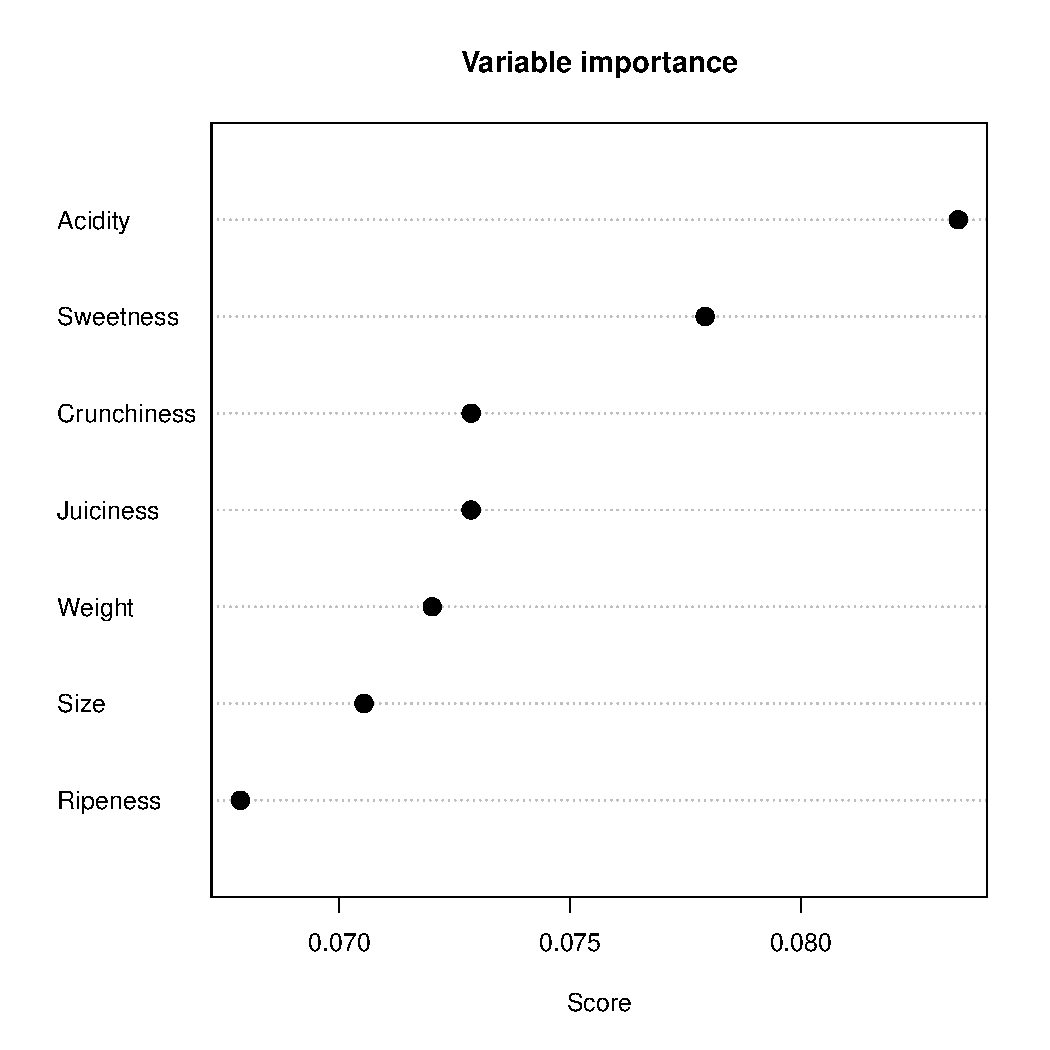
\includegraphics[width=0.9\columnwidth]{../r/plots/vip-adaboost-apple.pdf}
%\end{column}
%\hspace{-1.3ex}\begin{column}{0.515\textwidth}
%	% stochastic setting
%	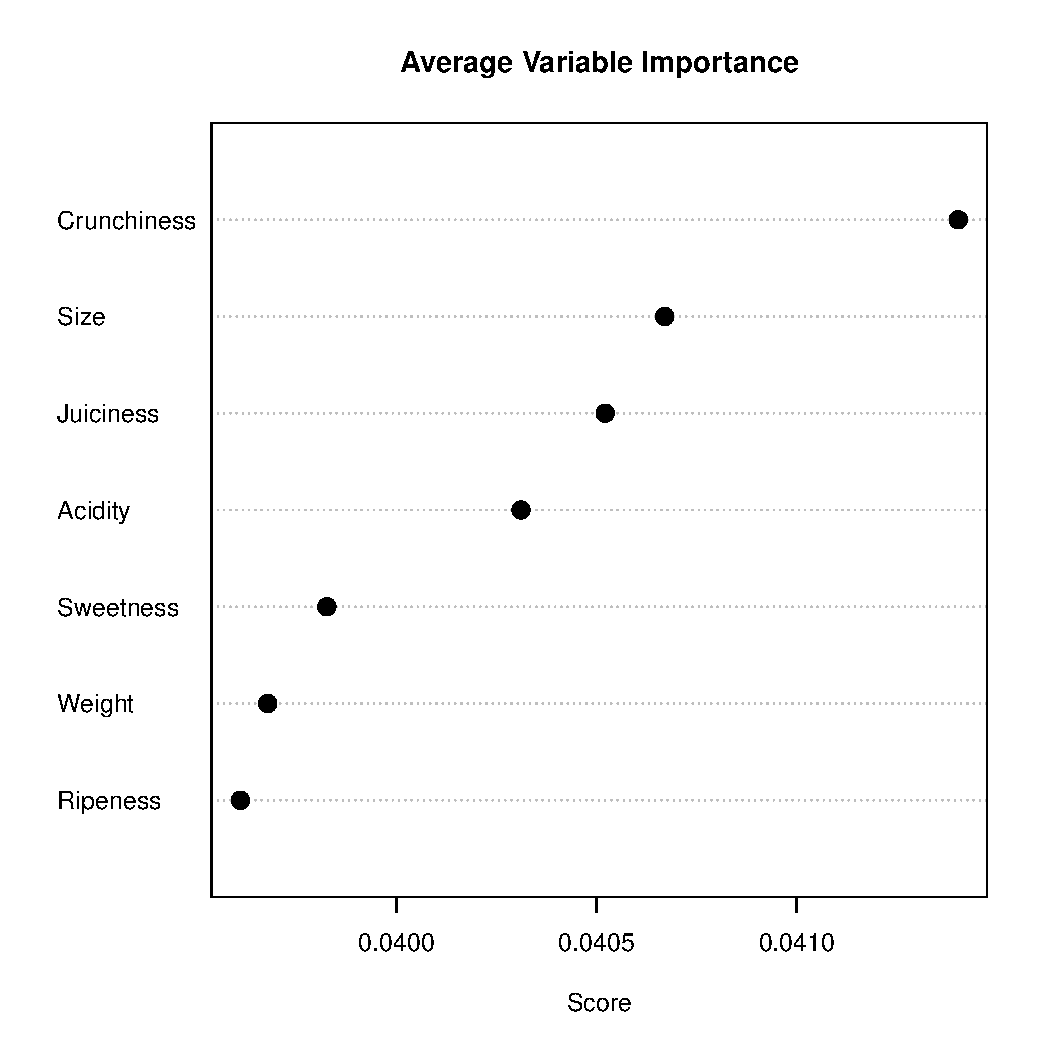
\includegraphics[width=0.9\columnwidth]{../r/plots/vip-adaboost-st1-apple.pdf}\vspace{-1em}
%	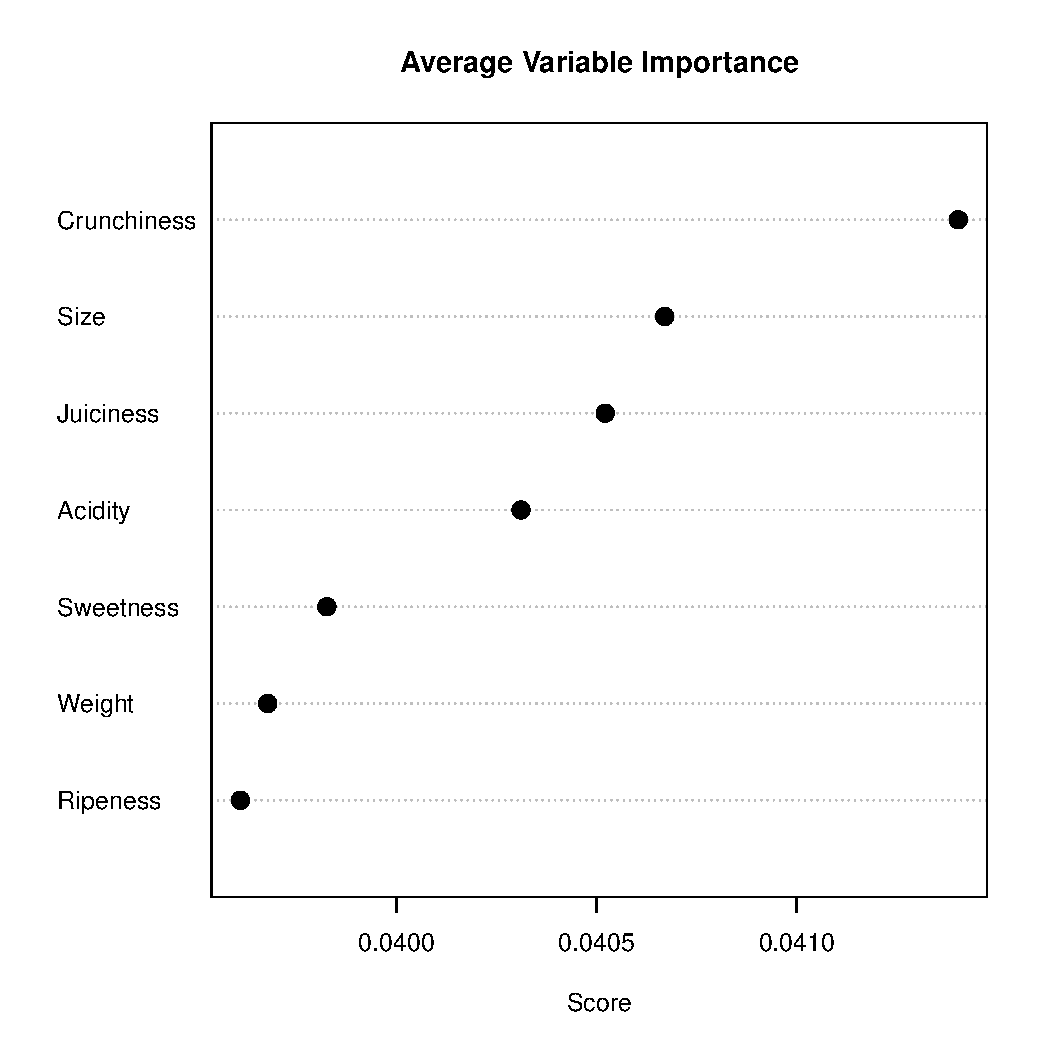
\includegraphics[width=0.9\columnwidth]{../r/plots/vip-adaboost-st1-apple.pdf}
%\end{column}
%\end{columns}
%
%\end{frame}

%\begin{frame}{Variable importance}
%
%\begin{figure}
%\hspace*{-3.2em}\begin{tikzpicture}
%%	\draw[help lines] (-5,-3) grid (6,3);\node[black,draw,circle] at (0,0) {};
%	% display anchors
%	\node[immagine] at (-5,-3) {\includegraphics[width=0.63\textwidth]{../r/plots/vip-adaboost-st0.pdf}};
%	\node[immagine,above left] at (8.2,-3) {\includegraphics[width=0.63\textwidth]{../r/plots/vip-adaboost-st1.pdf}};
%	
%	\draw[latex-latex,thick,bend left=10] (-3.4,2.4) to (1.6,-1.4);
%	\draw[latex-latex,thick,bend left=3] (-4.15,-1.4) to (1.6,1.8);
%
%	\node[draw,circle,thick,minimum size=0.4cm,mLightBrown] at (-4.48,-1.47) {};
%	\node[draw,circle,thick,minimum size=0.4cm,mLightBrown] at (1.92,1.88) {};
%
%	\node[draw,ellipse,thick,minimum width=1.2cm,mLightGreen] at (-4.1,2.45) {};
%	\node[draw,ellipse,thick,minimum width=1.2cm,mLightGreen] at (2.3,-1.45) {};
%\end{tikzpicture}
%\end{figure}
%
%\vspace{-1em}
%$M_{\text{max}}=1000$, $M^\ast=27$, $\lambda=1$, $\pi=0.5$
%
%\end{frame}

%\begin{frame}{Tuning}
%% error rate against rounds of boosting
%\begin{figure} % consider annotating M*
%\includegraphics[width=0.7\textwidth]{../r/plots/cv-adaboost.pdf}
%\end{figure}
%\end{frame}

%\begin{frame}{Variable importance}
%
%\begin{figure}
%\includegraphics[width=0.7\textwidth]{../r/plots/adaboost-varimp.pdf}
%\end{figure}
%
%\end{frame}

% !TeX spellcheck = en_GB

% ------------------------------- %

\begin{frame}{Metrics}

\begin{table}
\sisetup{round-mode=places}
\resizebox{\textwidth}{!}{
\begin{tabular}{lS[round-precision=3]S[round-precision=3]S[round-precision=3]S[round-precision=3]}
	\toprule
	& \multicolumn{2}{c}{Diabetes} & \multicolumn{2}{c}{Apple quality} \\
	Model & {Train score} & {Test score} & {Train score} & {Test score} \\
	\midrule
	AdaBoost & 0.875 & 0.76953125 & 0.93100862392201 & 0.86721680420105 \\
	$\text{AdaBoost}_\pi$ & 0.841796875 & 0.7578125 & 0.983127109111361 & 0.887471867966992 \\
	Model2 & 0. & 0. & 0. & 0. \\
	Model3 & 0. & 0. & 0. & 0. \\
	\bottomrule
\end{tabular}}
\end{table}

\end{frame}

% ------------------------------- %

% ------------------------------- %

%\appendix
%{\setbeamercolor{palette primary}{fg=black,bg=white}
%\begin{frame}[standout]
%%Thank you for your kindly attention!
%Questions?
%\end{frame}
%}

% ------------------------------- %


\appendix
\begin{frame}[allowframebreaks]{References}
\begin{thebibliography}{9}
	\bibitem{statslearn} T. Hastie, R. Tibshirani, and J. H. Friedman
	\newblock The Elements of Statistical Learning
	\newblock Springer, 6:191--199, 2009.
	% ---- %
	% add adaboost paper
	% add adaboost package
\end{thebibliography}
\end{frame}

% !TeX spellcheck = en_GB

\begin{frame}[fragile]{AdaBoost algorithm (Discrete AdaBoost)}

% gradient boosting
Discrete AdaBoost

{%
\setlength{\interspacetitleruled}{0pt}%
\setlength{\algotitleheightrule}{0pt}%
\begin{algorithm}[H]
\KwIn{$M$, $\set{(x_i,y_i)}_1^N$, $x_i\in\R^p$}
Initialize observation weights $w_i^{(1)}=1/N$ s.t. $\sum_{i=1}^Nw_i^{(m)}=1$\;
\For{$m=1$ \KwTo $M$}{
	Fit classifier $G_m(x)$ using $w_i^{(m)}$\;
	Weighted error rate $\text{err}_m=\sum_{i=1}^Nw_i^{(m)}\mathbb{I}(y_i\neq G(x_i))$\;
	Classifier's weight $\alpha_m=\log\bigl(\frac{1-\text{err}_m}{\text{err}_m}\bigr)$\;
	Observation weights $w_i^{(m+1)}\gets w_i^{(m)}\exp(\alpha_m\mathbb{I}(y_i\neq G(x_i)))$\;
}
\KwOut{$G(x)=\sign(\sum_{m=1}^M\alpha_mG_m(x))$}
\end{algorithm}}

%Where the \alert{weak learner} $G_m\in\set{-1,1}$ is a CART
Where the \alert{weak learner} $G_m\colon\R^p\to\set{-1,1}$ is a Decision Tree

% questa è la base di partenza
% poi è stato collegato a concetti statistici quali: loss function, modello additivo e regressione logistica
% è stato mostrato che discrete adaboost fitta una forward stagewise additive logistic regression che minimizza la exponential loss

\end{frame}

% ------------------------------- %

%\begin{frame}{Forward stagewise additive modeling}
%
%The general framework for boosting  % additive expansion of basis functions
%
%{%
%\setlength{\interspacetitleruled}{0pt}%
%\setlength{\algotitleheightrule}{0pt}%
%\begin{algorithm}[H]
%\KwIn{$M$, $\set{(x_i,y_i)}_1^N$}
%Start with $f_0(\boldsymbol{x})=0$\;
%\For{$m=1$ \KwTo $M$}{
%%	Solve
%	$(\beta_m,\gamma_m)=\argmin_{\beta,\gamma}\sum_{i=1}^NL(y_i,f_{m-1}(x_i)+\beta b(x_i;\gamma))$\;
%%	Update
%	$f_m(\boldsymbol{x})=f_{m-1}(\boldsymbol{x})+\beta_mb(\boldsymbol{x};\gamma_m)$\;
%}
%\end{algorithm}}
%
%Where $b(\boldsymbol{x};\gamma_m)\in\R$ is a basis function depending on parameter $\gamma_m$ %  the number of basis functions is chosen according to hyper-parameter M
%\end{frame}

% ------------------------------- %

\begin{frame}[fragile]{AdaBoost stochastic setting}
% stochastic setting
% stochastic gradient boosting framework, when bag.frac < 1
% -> shrinkage added
% -> out-of-bag fraction, on each iteration train a classifier on a different dataset sample, keep the rest as OOB

Discrete AdaBoost with shrinkage and out-of-bag, as an additive model with prediction function $f_m(x)$

{%
\setlength{\interspacetitleruled}{0pt}%
\setlength{\algotitleheightrule}{0pt}%
\begin{algorithm}[H]
\KwIn{$M$, $\set{(x_i,y_i)}_1^N$, $x_i\in\R^p$}
%Initialize observation weights $w_i^{(1)}=1/N$ s.t. $\sum_{i=1}^Nw_i^{(m)}=1$\;
Initialize $f_0(x)=0$\;
\For{$m=1$ \KwTo $M$}{
	Set $w_i^{(m)}=-\frac{\partial L(y,g)}{\partial g}\bigr\rvert_{g=f_m(x)}$ s.t.  $\sum_{i=1}^Nw_i^{(m)}=1$\;
	Fit classifier $G_m(x)$ using $w_i^{(m)}$ with samples from $\pi_m$\;
	Weighted error rate $\text{err}_m=\sum_{i=1}^Nw_i^{(m)}\mathbb{I}(y_i\neq G(x_i))$\;
	Set $\alpha_m=\frac{1}{2}\log\bigl(\frac{1-\text{err}_m}{\text{err}_m}\bigr)$\;
	Update $f_{m}(x)\gets f_{m-1}(x)+\lambda\alpha_mG_m(x)$\;
}
\KwOut{$G(x)=\sign(f_M(x))$}
\end{algorithm}}

\end{frame}


\end{document}
